\documentclass{article}
\usepackage[utf8]{inputenc}

\title{Introduction to Biological Imaging\\Homework}
\author{}%Johann Brenner, Mat. 03662733}
\date{Winter term 2018/19}

\usepackage[margin=2.8cm]{geometry}
\usepackage{color}
\definecolor{bisque}{rgb}{1.0, 0.89, 0.77}
\definecolor{mygreen}{rgb}{0,0.5,0}
\definecolor{mygray}{rgb}{0.5,0.5,0.5}
\definecolor{mymauve}{rgb}{0.58,0,0.82}
\usepackage{natbib}
\usepackage{graphicx} 	
\usepackage{listings}
\lstset{ 
	language=Matlab,                		% choose the language of the code
	%basicstyle=10pt,       				    % the size of the fonts that are used for the code
	numbers=left,                  			% where to put the line-numbers
	numberstyle=\tiny\color{mygray},        % the style that is used for the line-numbers
	stepnumber=1,                   		% the step between two line-numbers. If it's 1 each line will be numbered
	numbersep=5pt,                  		% how far the line-numbers are from the code
	backgroundcolor=\color{bisque},  	    % choose the background color. You must add \usepackage{color}
	commentstyle=\color{mygreen},           % comment style
	deletekeywords={...},                   % if you want to delete keywords from the given language
	keywordstyle=\color{blue},              % keyword style
	morekeywords={*,...,ifftshift},         % if you want to add more keywords to the set
	showspaces=false,               		% show spaces adding particular underscores
	showstringspaces=false,         		% underline spaces within strings
	showtabs=false,                 		% show tabs within strings adding particular underscores
	frame=single,	                		% adds a frame around the code
	tabsize=2,                				% sets default tabsize to 2 spaces
	captionpos=b,                   		% sets the caption-position to bottom
	breaklines=true,                		% sets automatic line breaking
	breakatwhitespace=false,        		% sets if automatic breaks should only happen at whitespace
	escapeinside={\%*}{*)},          		% if you want to add a comment within your code
	stringstyle=\color{mymauve}             % string literal style
}
\usepackage{pdfpages}
\usepackage{enumitem}
\usepackage{amsmath}
\usepackage{siunitx}
\usepackage{subcaption}
\usepackage[T1]{fontenc}
\usepackage{textcomp}
\usepackage{titlesec}
%\newcommand{\sectionbreak}{\clearpage}
\newcommand\subsectionbreak{\ifnum\value{subsection}>1\clearpage\fi}
\newcommand{\sectionbreak}{\clearpage}
\titleformat{\chapter}[display]
  {\normalfont\bfseries}{}{0pt}{\Huge}
%\renewcommand\thesubsection{\alph{subsection}}

\usepackage{fancyhdr}
\pagestyle{fancy}
\fancyhf{}
%\fancyhead[c]{Johann Brenner - Mat.-Nr. 03662733}
\fancyfoot[c]{\thepage}

\begin{document}

    \maketitle
    
    \tableofcontents    
     \section{Homework 1}
     \subsection*{Assignment 1}
\addcontentsline{toc}{subsection}{Assignment 1}
In the following, the code to answer the questions of the first assignment is plotted.

\subsubsection*{Task 1}
\addcontentsline{toc}{subsubsection}{Task 1}
\begin{lstlisting}
%% 1) Create a phantom for simulating XCT measurements.
% The phantom should contain % ellipses and polygons of varying intensity
% (use phantom() and augment the resulting
% image). Show an image of your phantom.
% Size of quadratic Phantom in pixels
img_width = 256;
img_length = img_width;
% Determine Ellipe count (min = 3)
num_ellipses = 6;
% Initialize array
E = zeros(num_ellipses,6);
% Get basic skull structure from phantom
[~,base] = phantom('Modified Shepp-Logan', img_width);
E(1:2,:) = base(1:2,:);
% Get remaining array size
[M,N] = size(E(3:end,:));
% Create random ellipse along boundaries
E(3:end,1) = rand(M,1);
E(3:end,2) = -0.2 + (0.3+0.3)*rand(M,1);
E(3:end,3) = -0.4 + (0.4+0.4)*rand(M,1);
E(3:end,4) = -0.4 + (0.4+0.4)*rand(M,1);
E(3:end,5) = -0.45 + (0.45+0.45)*rand(M,1);
E(3:end,6) =  180*rand(M,1);
% Build phantom only of ellipses
phntm = phantom(E,img_width);
% Increase inensity of pixels in a square of the matrix
phntm(img_width/2-16:img_width/2+16,img_width/2-16:img_width/2+16) =...
    phntm(img_width/2-16:img_width/2+16,img_width/2-16:img_width/2+16) + 0.5;
% visualize the phantom
figure; imagesc(phntm);
axis equal tight; colormap gray; colorbar; xlabel('x'); ylabel('y');
title('Random Shepp-Logan Phantom');
\end{lstlisting}
\newpage

\begin{figure}[htb!]
    \centering
    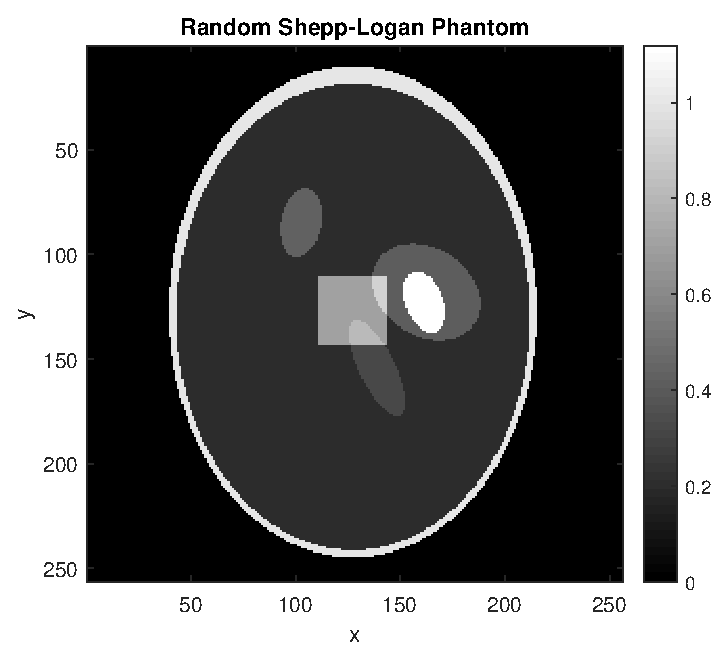
\includegraphics[width=\linewidth]{homework1/img/10.eps}
    \caption{Randomly generated skull}
    \label{fig:rand_skull}
\end{figure}

\clearpage
\newpage
\subsubsection*{Task 2}
\addcontentsline{toc}{subsubsection}{Task 2}

\begin{lstlisting}
%% 2) Compute the views (projections) for the range of angles from 0 to 179 degrees with spacing
% of 1, 5 and 10 degrees. Show the projections at 0, 30, 45 and 90 degrees (in one axes). Show the
% sinogram with the most angles/projections.
% specify projection angles
theta = {0:1:179;
    0:5:179;
    0:10:179}; 
% pad the image with zeros so nothing gets lost during rotation
img_diag = sqrt(img_length^2 + img_width^2);
padding = ceil(img_diag - img_width) + 4;
pad_img = zeros(img_length + padding, img_width + padding);
pad_img(ceil(padding/2):(ceil(padding/2) + img_length - 1),...
    ceil(padding/2):(ceil(padding/2) + img_width - 1)) = phntm;
% loop over the number of angles and summarize
th = theta{1};
n = length(th);
img_pr = zeros(size(pad_img,2), n);
for i = 1:n
    tmp_img = imrotate(pad_img,180+th(i), 'bilinear', 'crop');
    img_pr(:,i) = (sum(tmp_img))';
end
% create a sinograms for the specified angles
for i = 1:length(theta)
sinogram{i}(:,:) = radon(phntm, theta{i}); 
end
% Plot sinogram data at specific points in the same axes
figure;
plot(sinogram{1}(:,1),'DisplayName',[num2str(theta{1}(:,1))  ' degrees']);
hold on
plot(sinogram{1}(:,31),'DisplayName',[num2str(theta{1}(:,31)) ' degrees']);
plot(sinogram{1}(:,46),'DisplayName',[num2str(theta{1}(:,46)) ' degrees']);
plot(sinogram{1}(:,91),'DisplayName',[num2str(theta{1}(:,91)) ' degrees']);
title('Radon Transform at specific angles'); legend
% visualize the sinogram
figure; 
imagesc(sinogram{1}); 
title(['Sinogram @ ' num2str(length(theta{1})) 'angles (' num2str(theta{1}(:,1)) '\textdegree -' num2str(theta{1}(:,end)) '\textdegree)']);
xlabel('Angle');colormap gray;colorbar
\end{lstlisting}

\begin{figure}[htb!]
    \centering
    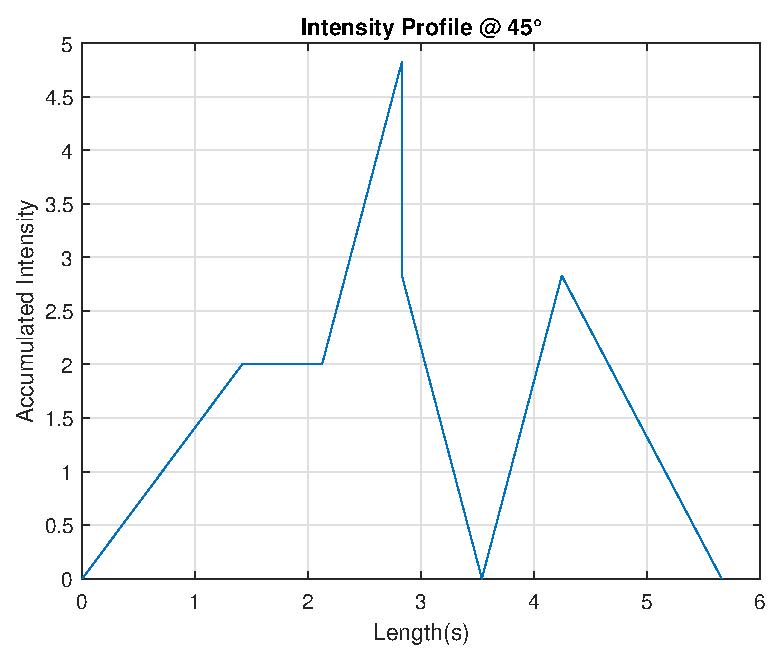
\includegraphics[width=.6\linewidth]{homework1/img/8.eps}
    \caption{Sinogram with the most angles (180)}
    \label{fig:sinogram:compl_angles}
\end{figure}

\begin{figure}[htb!]
    \centering
    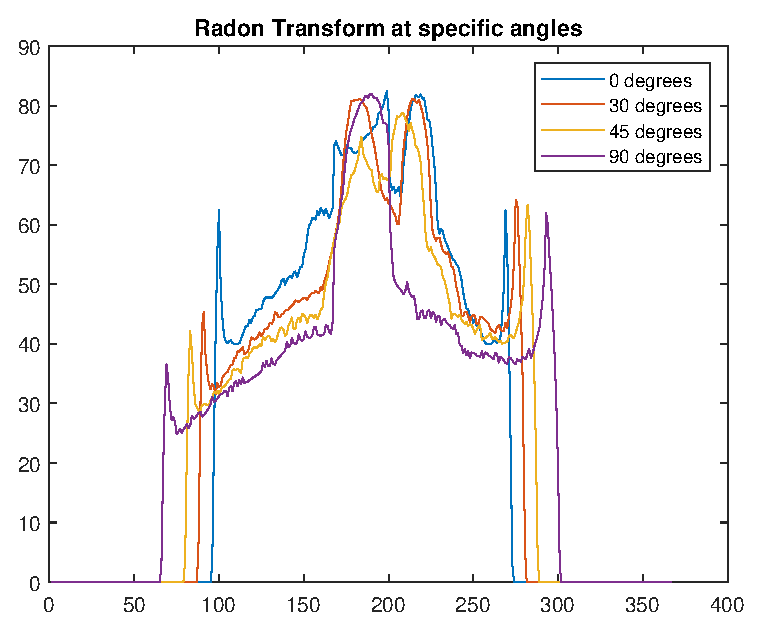
\includegraphics[width=.6\linewidth]{homework1/img/9.eps}
    \caption{Projections at the specific angles}
    \label{fig:sinogram:spec_angles}
\end{figure}

\clearpage
\newpage

\subsubsection*{Task 3}
\addcontentsline{toc}{subsubsection}{Task 3}

The following code was implemented as a seperate MATLAB function, in order to reduce the amount and simplify the code.

\begin{lstlisting}
%%%%%%%%%%%%%%%%%%%%%%%%%%%%%%%%%%%%%%%%%%%%%%%%%%%%%%%%%%%%%%%%%%%%%%%%%%%
%% Backprojection Algorithm %%
%%%%%%%%%%%%%%%%%%%%%%%%%%%%%%%%%%%%%%%%%%%%%%%%%%%%%%%%%%%%%%%%%%%%%%%%%%%
% Parameters: 
% sinogram: Input 2D - sinogram matrix
% theta: corresponding angles of sinogram
% filter_shape('none','Ramp','Cos','Hamming'): Selection of applied filter
% method
% Output: 
% rec: Reconstructed image
function rec = backprojection(sinogram,theta,filter_shape)
if nargin <3
    filter_shape = 'none';
end
% figure out how big the picture is going to be.
sideSize = size(sinogram,1); 
%filter setups
x = linspace(-1,1,sideSize);
ramp = abs(x);
switch filter_shape
    case 'Ramp'
        filter = ramp;
    case 'Hamming'
        filter = ramp .* hamming(sideSize)';
    case 'Cos'
        filter = ramp .* cos((x./2).*pi).^2;
    otherwise
        filter = 1;
end
% set up the image
rec = zeros(sideSize,sideSize);
for i = 1:length(theta)    
    line = sinogram(:,i);    
    % perform fft
    line_fft = fftshift(fft(ifftshift(line)));        
    % filter in frquency space
    line_fft_filtered = line_fft .* filter';    
    % transform back into time domain
    line_filtered = ifftshift(ifft(fftshift(line_fft_filtered)));    
    % backproject
    image = repmat(line_filtered,1,sideSize);
    image = imrotate(image,theta(i),'crop');    
    % sum up final picture
    rec = rec + image;
end
% rotate image as the original
rec = real(imrotate(rec,90))./length(theta);
end
\end{lstlisting}


\clearpage
\newpage


\subsubsection*{Task 4}
\addcontentsline{toc}{subsubsection}{Task 4}

\begin{lstlisting}
%% 4) Reconstruct the phantom data with the specified angular spacings using your
% backprojection algorithm without filtering. Show the obtained reconstructions.
recon = backprojection(sinogram{1},theta{1});
% visualize reconstruction results
figure;
subplot(1,2,1);
imagesc(phntm);
axis equal tight;
colormap gray;
title('Original'); xlabel('x'); ylabel('y');
subplot(1,2,2);
imagesc(recon);
axis equal tight;
colormap gray;
title('Unfiltered BP'); xlabel('x'); ylabel('y');
\end{lstlisting}
\begin{figure}[htb!]
  \centering
  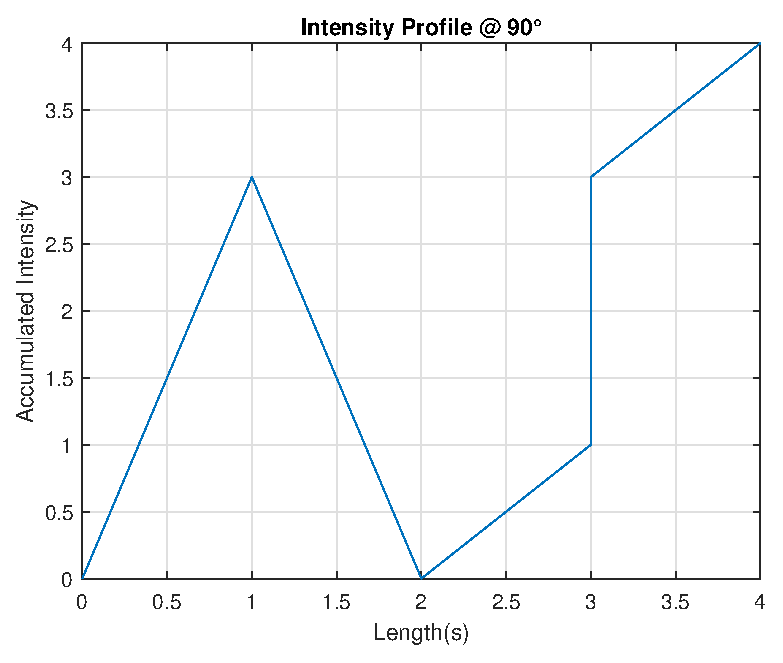
\includegraphics[width=\linewidth]{homework1/img/7.eps}
  \caption{Reconstruction from 1\textdegree resolution without any filtering}
  \label{fig:recon_1deg}
\end{figure}

\clearpage
\newpage


\subsubsection*{Task 5}
\addcontentsline{toc}{subsubsection}{Task 5}

\begin{lstlisting}
%% 5) Incorporate filtering in your backprojection. Implement 3 filters (ramp, cosine and
% hamming) and test their influence on the reconstruction using your phantom data (pick
% a single angle spacing). Show the reconstruction results
for i = 1:3
    % Compute filtered backprojections
    recon_cos = backprojection(sinogram{i},theta{i},'Cos');
    recon_ramp = backprojection(sinogram{i},theta{i},'Ramp');
    recon_hamming = backprojection(sinogram{i},theta{i},'Hamming');
    % visualize reconstruction results
    figure;
    subplot(2,2,1);
    imagesc(phntm);
    title(['w/o Filtering,' num2str(length(theta{i})) ' angles']);
    colormap gray; colorbar; xlabel('x'); ylabel('y');
    subplot(2,2,2);
    imagesc(recon_ramp);
    title(['w/ Ramp Filtering, ' num2str(length(theta{i})) ' angles']);
    colormap gray; colorbar; xlabel('x'); ylabel('y');
    subplot(2,2,3);
    imagesc(recon_hamming);
    title(['w/ Hamming Filtering, '  num2str(length(theta{i})) ' angles']);
    colormap gray; colorbar; xlabel('x'); ylabel('y');
    subplot(2,2,4);
    imagesc(recon_cos);
    title(['w/ Cosine Filtering, ' num2str(length(theta{i})) ' angles']);
    colormap gray; colorbar; xlabel('x'); ylabel('y');
end
\end{lstlisting}

\begin{figure}[htb!]
  \centering
  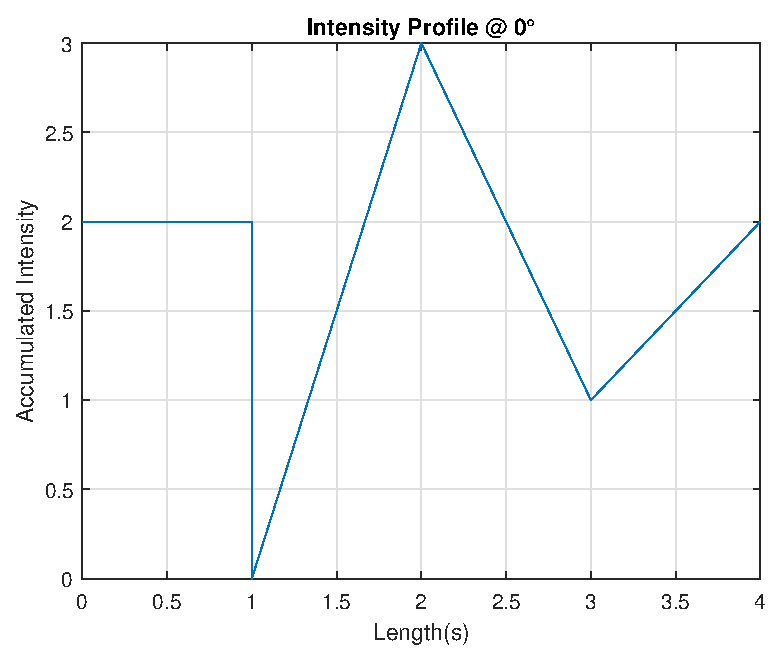
\includegraphics[width=\linewidth]{homework1/img/6.eps}
  \caption{1\textdegree resolution}
  \label{fig:recon_1deg}
\end{figure}
\begin{figure}[htb!]
  \centering
  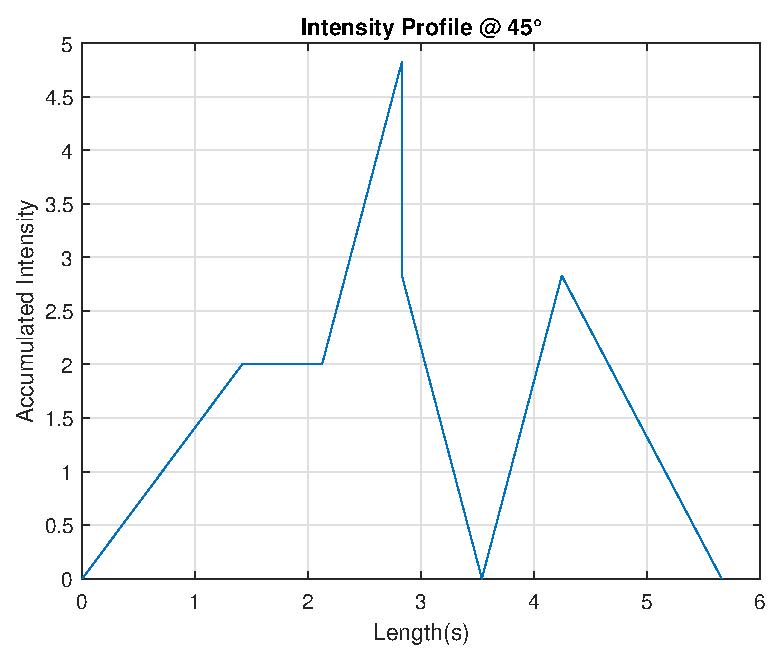
\includegraphics[width=\linewidth]{homework1/img/5.eps}
  \caption{5\textdegree resolution}
  \label{fig:recon_5deg}
\end{figure}
\begin{figure}[htb!]
  \centering
  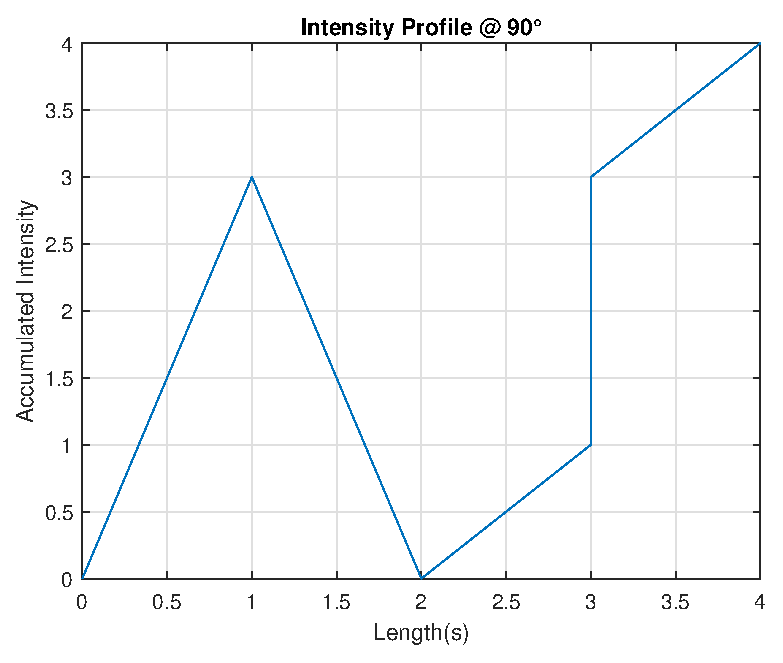
\includegraphics[width=\linewidth]{homework1/img/4.eps}
  \caption{10\textdegree resolution}
  \label{fig:recon_10deg}
\end{figure}


\clearpage
\newpage


\subsubsection*{Task 6}
\addcontentsline{toc}{subsubsection}{Task 6}

\begin{lstlisting}
%% 6) Reconstruct the provided datasets (CT_2018.mat) with your backprojection algorithm
% without filtering and with each of the implemented filters, respectively. Show the
% reconstructed images.

% load sample data
S = load('CT_2018.mat');
% loop over sample data, compute backprojections and plot them each in a
% single figure
for i = 1:3
    % change variable name dynamically
    sino_name = S.(['sino' num2str(i-1)]);
    angle = S.(['theta' num2str(i-1)]);
    % visualize
    fig_name = sprintf('%s with %d angles from %d° to %d°', ['sino' num2str(i-1)],length(angle), angle(1),angle(end));
    figure('Name',fig_name);
    subplot(2,2,1);
    recon = backprojection(sino_name,angle);
    imagesc(recon);
    title('w/o Filtering');
    colormap gray; colorbar; xlabel('x'); ylabel('y');
    subplot(2,2,2);
    recon = backprojection(sino_name,angle,'Ramp');
    imagesc(recon);
    title('w/ Ramp Filtering');
    colormap gray; colorbar; xlabel('x'); ylabel('y');
    subplot(2,2,3);
    recon = backprojection(sino_name,angle,'Hamming');
    imagesc(recon);
    title('w/ Hamming Filtering');
    colormap gray; colorbar; xlabel('x'); ylabel('y');
    subplot(2,2,4);
    recon = backprojection(sino_name,angle,'Cos');
    imagesc(recon);
    title('w/ Cosine Filtering');
    colormap gray; colorbar; xlabel('x'); ylabel('y');
end
\end{lstlisting}

\begin{figure}[htb!]
  \centering
  \includegraphics[width=\linewidth]{homework1/img/3.eps}
  \caption{1\textdegree resolution}
  \label{fig:recon_1deg}
\end{figure}
\begin{figure}[htb!]
  \centering
  \includegraphics[width=\linewidth]{homework1/img/2.eps}
  \caption{2\textdegree resolution}
  \label{fig:recon_5deg}
\end{figure}
\begin{figure}[htb!]
  \centering
  \includegraphics[width=\linewidth]{homework1/img/1.eps}
  \caption{0.5\textdegree resolution}
  \label{fig:recon_10deg}
\end{figure}

\clearpage
\newpage


\subsubsection*{Task 7}
\addcontentsline{toc}{subsubsection}{Task 7}

\textbf{Shortly interpret your results:}
\begin{enumerate}[label=(\alph*)]

\item What is the effect of different angular spacings on the reconstruction?\\
Finer Spacings <==> More Information, therefore better reconstruction, more details visible.

\item How do the different filters change the reconstruction results?\\
Filters affect the edge sharpness, the residual noise and the overall brightness of an image

\item Which filter performs best? Why? Under which circumstances?\\
The Hamming filter performs best overall, because he does not damp the low frequencies to zero,as cosine and ramp filter do.
\end{enumerate}

\begin{enumerate}[label=(\alph*)]
    \item What is the effect of different angular spacings on the reconstruction?\\
    Finer spacing provide more information, therefore a better reconstruction is possible.
    \item How do the different filters change the reconstruction results?\\
    Different filters affect different radial resolutions. They either provide more or less noise.
    \item Which filter performs best? Why? Under which circumstances?\\
    In the case of the self-made phantom, the Hamming filter performs best due to its elaborate filtering function. In comparison of the three filters the hamming flter is a good compromise between high contrast and noise. The cos filter looses a lot of information for low frequencies. Filtering is always a trade off between reducing the noise and getting a high resolution.
\end{enumerate}


     \subsection*{Assignment 2}
\addcontentsline{toc}{subsection}{Assignment 2}
Assume the 2x2 discretization of the spatial distribution of absorption coefficient shown in Fig. 1 and 2 point detectors with spacing L.

\subsubsection*{Task 1}
\addcontentsline{toc}{subsubsection}{Task 1}
Design a model matrix A that relates X-ray measurements $p= (p_1, p_2, p_3, p_4, p_5, p_6)^T$ at 3 shown angles to the (unknown) absorption $\mu= (\mu_1, \mu_2, \mu_3, \mu_4)^T$ as in: $ \mathbf{A} \mathbf{µ} = \mathbf{p} $. Show A.

\begin{lstlisting}
%% 1) Design a model matrix A that relates X-ray measurements 
% p=(P1,P2,P3,P4,P5,P6)T at 3 shown angles to 
% the (unknown) absorption mu=(mu1,mu2,mu3,mu4)T as in: A*mu = p. Show A.

% scaling for 45° beams
a = sqrt(2) - 1; 

syms L;

% setup model matrix
A = [L, 0, L, 0;
0, L, 0, L;
a*L, 0, L, a*L;
a*L, L, 0, a*L;
0, 0, L, L;
L, L, 0, 0];

pretty(A);
\end{lstlisting}

\begin{equation}
    \mathbf{A} = \left(\begin{array}{cccc} L & 0 & L & 0\\ 0 & L & 0 & L\\ (\sqrt{2} - 1)L & 0 & L &  (\sqrt{2} - 1)L \\  (\sqrt{2} - 1)L  & L & 0 &  (\sqrt{2} - 1)L \\ 0 & 0 & L & L\\ L & L & 0 & 0 \end{array}\right)
\end{equation}


\subsubsection*{Task 2}
\addcontentsline{toc}{subsubsection}{Task 2}
\begin{lstlisting}
%% 2) Assume a specific distribution (values) of mu_test and a specific value of L
% Simulate the corresponding measurements mu_test for this distribution
% using the model matrix A. Show p_test.

L_spec = 4;
A_subs = double(subs(A,L,L_spec));
mu_test = rand([4,1]); % assume (random) values of absorption mu

p_test = A_subs*mu_test % simulate corresponding measurements b
\end{lstlisting}

\begin{equation}
    P = \left(\begin{array}{c}
    5,13361736274707\\6,49676346881041\\5,18217061046964\\5,35509078478611\\6,32384329449394\\5,30653753706355 \end{array}\right)
\end{equation}



\subsubsection*{Task 3}
\addcontentsline{toc}{subsubsection}{Task 3}
\begin{lstlisting}
%% 3) Using the simulated measurements p_test, reconstruct absorption mu_rec,
% i.e. solve A*mu_rec=p_test. Show both the assumed (mu_test) and
% the reconstructed (mu_rec) absorption distributions.

% now we try to recover mu back from our measurements:
% A*mu = p => mu = inv(A)*p - we try to solve for mu that is assumed unknown
% inv(A)*p % doesn't work, rank of A is 3!

mu_rec = lsqr(A_subs, p_test); % min||A*mu-p||.^2 - we try to find a solution using minmization procedure
rel_error_perc = abs(mu_test - mu_rec)./mu_test*100 % looking at the relative error in percent, we're pretty far off from the real values
\end{lstlisting}

\begin{align*}{4}
    \mu_{rec}  &= \left(\begin{array}{c} 0,647617630172602\\0,679016754093115\\0,635786710513997\\0,945174113109320 \end{array}\right)\\
    \mu_{test} &= \left(\begin{array}{c} 0,647617630172602\\0,679016754093115\\0,635786710513997\\0,945174113109320 \end{array}\right)\\
    rel-error-perc &= \left(\begin{array}{c} 1.2703\cdot 10^{-11}\\ 1.2796\cdot 10^{-11}\\ 1.3672\cdot 10^{-11}\\ 8.6099\cdot 10^{-12} \end{array}\right)
\end{align*}


\subsubsection*{Task 4}
\addcontentsline{toc}{subsubsection}{Task 4}
\begin{enumerate}[label=(\alph*)]
    \item Does the reconstruction $\mu_\text{rec}$ correspond to the assumed distribution mutest of the absorption coefficient?\\
    According to variable rel-error-perc, $\mu_{rec}$ matches the array $\mu_{test}$ at a relative error smaller than 1E-10 percent. This means, the arrays can considered to be the same.
    \item Did you use inv() for inverting the model? Why?\\
     No, because model matrix a A is no square matrix and has a rank of 4.
\end{enumerate}

     \section{Homework 2}
     \subsection{Finite Difference Method}
\subsubsection{Come up with a simple one dimensional differential equation \\$\mathbf{f'(x)=g(x)\ \mathrm{on}\ \Omega=[0,1]}$ by specifying g(x) and setting appropriate boundary condition (e. g. $\mathbf{f(0) = 0}$).}
Initial assumption:
\begin{equation}
    g(x) = \cos^2(\pi x)
\end{equation}
Dirichlet boundary condition:
\begin{align}
    f(0) &= 0 \label{eq:bcs}
\end{align}

\subsubsection{Solve the obtained boundary value problem analytically. Show your solution as well
as its plot.}
\begin{align}
   \int{f'(x)\ dx} &= \int{\cos^2(\pi x)\ dx}\\
  f(x) &= \frac{x}{2}+\frac{\sin\left(2\,\pi \,x\right)}{4\,\pi } + c_1\\
  f(0) &= \frac{0}{2}+\frac{\sin\left(2\,\pi \,0\right)}{4\,\pi } + c_1 \overset{!}{=} 0\\
  \Rightarrow c_1 &= 0
\end{align}
\clearpage
The corresponding MATLAB code was imeplemented as follwing:
\begin{lstlisting}
x_cont = linspace(0,1,1000);
x_interval = [0,1];
%% Plot ODE f'(x) = cos(pi x)^2 and its solution
syms f(x)
ODE = diff(f,x) == (cos(pi.*x)).^2;
bc = f(0) == 0;
sol = dsolve(ODE,bc);

figure;
yyaxis right
plot(x_cont,(cos(pi.*x_cont)).^2,'DisplayName',['ODE (f''(x) ='...
    'cos(x \pi)^2)']); hold on
xlabel('x');
ylabel('f''(x)');
yyaxis left
fplot(sol,x_interval,'DisplayName',['Analytical Solution '...
    '(f(0)=0, ' newline 'f(x)=^{x}/_{2}+sin(2\pix)/4\pi )']);
legend;
xlabel('x');
ylabel('f(x)');
\end{lstlisting}
\begin{figure}[htb!]
    \centering
    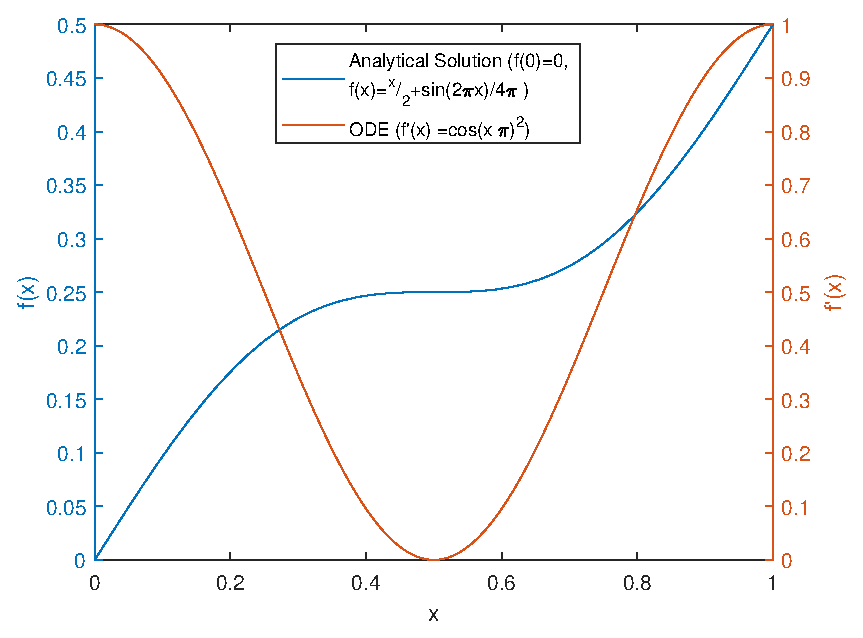
\includegraphics[width=.7\linewidth]{./homework2/img/1.eps}
    \caption{Original ODE with analytical solution}
    \label{fig:ana_sol}
\end{figure}
\subsubsection{Solve the boundary value problem using the Finite Difference Method for step h =
0.2, 0.1 and 0.01. Pick the discretization scheme yourself (forward/backward/central
difference), discretize the equation and put it into matrix form. Use linsolve() to solve
the resulting system of linear equations. Hint: unless you know what you are doing,
avoid central difference scheme.}
Choosing the \textit{forward Method} for the Finite Differences Method, where $x_i = i\ \cdot\ h\ \mathrm{with}\ i = 1,2,..., N+1\ \mathrm{and}\ N + 1= \frac{1}{h}$. 
For given h values of 0.2, 0.1 and 0.01 the dimension $M$ is 5, 10 and 100.
\begin{align}
    f'(x) &= \lim\limits_{h \rightarrow 0}{\frac{f(x+h)-f(x)}{h}}\\
    \frac{f(x+h)-f(x)}{h} &= \cos^2(\pi x) \\
    \mathrm{Discretizing:}\ \frac{f(x_{i+1})-f(x_i)}{h} &= \cos^2(\pi x_i)\\
    \mathrm{Rewriting:}\ f(x_{i+1})-f(x_i) &= h\cos^2(\pi x_i)\\
    \mathrm{Using\ Eq.}\ \ref{eq:bcs}:\ f_{1} &= f(0) = 0\\
    \underbrace{\begin{bmatrix}
    1 &   &   &   &   &   &   &   &  0\\
    -1 &  1 &   &   &   &   &   &  & \\
       &    &   &   &   &   &   &   &  \\
       &    &   &   &   &   &   &   &  \\
       &    &   &   &\ddots &\ddots &   &   &  \\
       &    &   &   &   &   &   &   &  \\
       &    &   &   &   &   &   &   &  \\
       &    &   &   &   &   &-1 &  1& \\
     0 &    &   &   &   &   &   &-1 &1\\
    \end{bmatrix}}_{M\times M}
    \underbrace{\begin{bmatrix}
f_2 \\f_3 \\ \\ \\ \vdots\\ \\ \\f_{N-1}\\ f_{N}
\end{bmatrix}}_{M\times 1}&= h \underbrace{\begin{bmatrix}
\cos^2(\pi x_1)\\\cos^2(\pi x_2)\\ \\ \\ \vdots \\ \\ \\\cos^2(\pi x_{N-2})\\\cos^2(\pi x_{N-1})
\end{bmatrix}}_{M\times 1}
\end{align}
\clearpage
The Finite Differences were computed by the following MATLAB script:
\begin{lstlisting}
%% Finite Difference Method
% Initialize Matrices
h = [0.2 0.1 0.01];
mat_size = 1./h;
A = cell(length(mat_size),1);
b = cell(length(mat_size),1);
f = cell(length(mat_size),1);
x = cell(length(mat_size),1);
fin_diff = cell(length(mat_size),1);

figure;
fplot(sol,x_interval,'DisplayName','Analytical Solution');hold on
% Populate A and b
for i = 1:length(mat_size)
    x{i} = linspace(0,1,mat_size(i))';
    A{i} = eye(mat_size(i));
    for j = 2:(mat_size(i))
        A{i}(j,j-1) = -1;
    end
    
    b{i} = double(h(i) .* ones(mat_size(i),1) .* (cos(pi .* x{i})).^2);
    
    % Evaluate Af = b
    f{i} = linsolve(double(A{i}),b{i});
    
    % Plot solution
    plot(x{i},[0;f{i}(1:end-1)],'DisplayName',['Finite Difference h = ' num2str(h(i))]);
end
legend({},'Location','northwest');
xlabel('x_i');
ylabel('f(x_i)');
\end{lstlisting}
\clearpage
\subsubsection{Plot the resulting solutions along with the exact solution you have computed in step 2}
\begin{figure}[htb!]
    \centering
    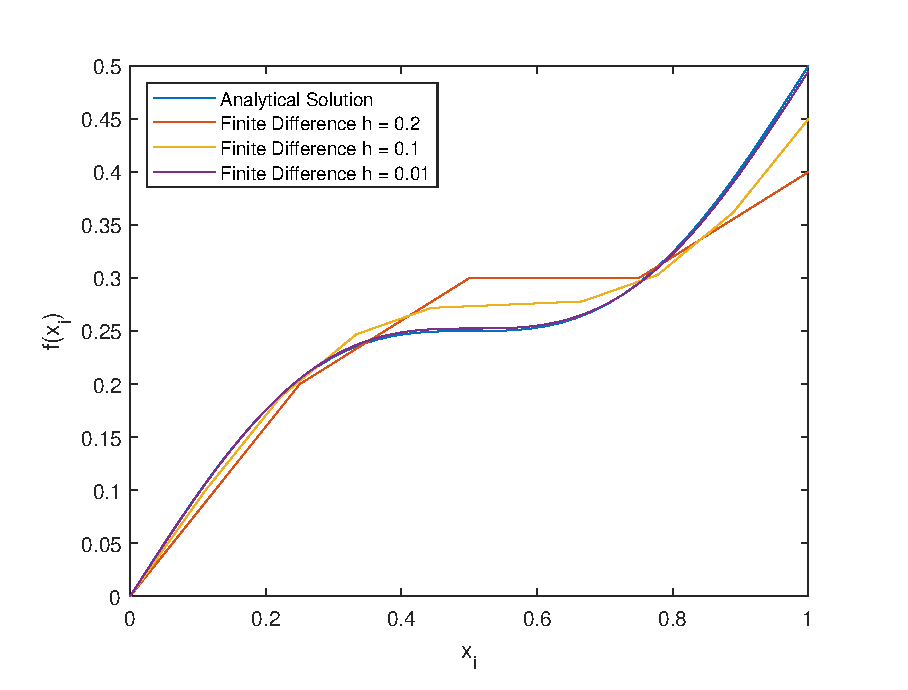
\includegraphics[width=.7\linewidth]{./homework2/img/final_FDM.eps}
    \caption{Analytical and Finite Difference solutions of the ODE}
    \label{fig:fin_diff}
\end{figure}
     \subsection{Assignment 2. Finite Element Method}
\subsubsection{Derive quadratic interpolation functions for the finite element method. Plot them in local coordinates. Show your derivation.}
As shown in the lecture, for the square shape functions, we can write our trial solution as:
\begin{align}
\widehat{T} &= a_0 + a_1 x +a_2 x^{2}\\
     &= \underbrace{\begin{bmatrix}1 & x & x^2\end{bmatrix}}_{X} \underbrace{\begin{bmatrix}a_0 & a_1 & a_2\end{bmatrix}^T}_{A}\\
    T_{i_{1}} &= T(0) = a_0 + a_1 \cdot 0 + a_2 \cdot 0^2\\
    T_{i_{2}} &= T(1/2) = a_0 + \frac{a_1}{2} + \frac{a_2}{2^2}\\
    T_{i_{3}} &= T(1) = a_0 + a_1 \cdot 1+a_2 \cdot 1^2  \\
    \underbrace{\begin{bmatrix}T_{i_1} \\ T_{i_2} \\ T_{i_3}\end{bmatrix}}_{T} &=
         \underbrace{\begin{bmatrix}
         1 & 0 & 0\\
         1 & \frac{1}{2} & \frac{1}{2^2}\\
         1 & 1 & 1\end{bmatrix}}_{L}
         \underbrace{\begin{bmatrix}a_0 \\ a_1 \\ a_2\end{bmatrix}}_{A} \\
         XA &= NLA\\
         N &= XL^{-1}\\
         &= \begin{bmatrix} 2\,x^2-3\,x+1 & 4\,x-4\,x^2 & 2\,x^2-x \end{bmatrix}
\end{align}
\begin{figure}[htb!]
    \centering
    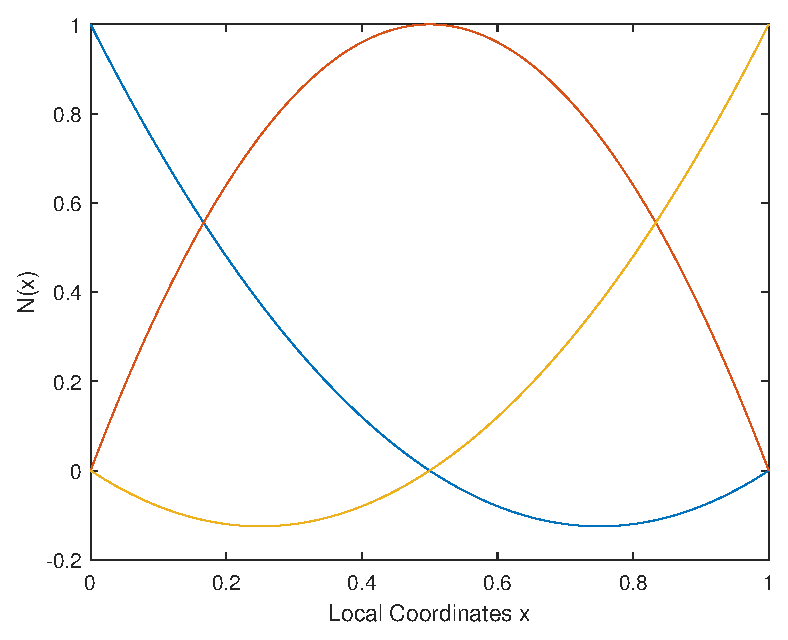
\includegraphics[width=.7\linewidth]{./homework2/img/3.eps}
    \caption{Quadratic FEM Interpolation Functions}
    \label{fig:interpol_functions}
\end{figure}

\subsubsection{ Consider a 1D steady state heat conduction problem, where $k$ and $S$ are constant. How would the stiffness matrix for one element look like for the shape functions derived in step 1?}
Problem:
\begin{align}
    kT'' + S &= 0\ \mathrm{on}\ \Omega \in [0,1]\\
    T(0) = &0,\ T(1) = 0 \\
    k_{stiff}(i,j) &= \int_{0}^{1}{N'(i) \cdot N'(j) dx}\\
    k_{stiff} &= \begin{bmatrix}
    2.\bar{3} & -2.\bar{6} &  0.\bar{3} \\
    -2.\bar{6} &  5.\bar{3} & -2.\bar{6} \\
    0.\bar{3} & -2.\bar{6} &  2.\bar{3}\end{bmatrix}
\end{align}
\begin{lstlisting}
%% 3D Finite Element Method

% Local x
x_local = 0:0.01:1;
L = [1,0,0; 1,0.5,0.25;1,1,1];
L_inv = inv(sym(L));

syms x
X = [1,x,x^2];
N = X*L_inv;

figure; %visualize cubic shape functions
for i = 1:length(N)
    plot(x_local, subs(N(i),x_local),'DisplayName',['Square Shape Function ' num2str(i)]); hold on;
end
xlabel('Local Coordinates x');
ylabel('N(x)');
%% Stiffness Matrix
k_stiff = zeros(length(N));

for i = 1:length(N)
    for j = 1:length(N)
        k_stiff(i,j) = double(int( diff(N(i), x).*diff(N(j), x), x, 0, 1 ));
    end
end

nodes = 3; % number of elements
Ke = double(k_stiff);
RHSe = int(N, x, 0, 1)';


L = 1; % domain length
k = 1; %for k = [100,10,1,0.1] %; % thermal conductivity,1
S = 10; %    for S = [100,10,1,0.1]% % source,100
l = L/nodes; % node spacing assuming equidistant nodes
dim = nodes*(nodes - 1) +1; %dimension of stiffness matrix
K = zeros(dim); %initialize stiffness matrix with zeros
RHS = zeros([dim, 1]); %initialize load vector with zeros

for i = 1:nodes %cycle through elements
    
    %compute indices of entries for a given element
    ind_start = 1+(i-1)*(nodes-1);
    ind_end = ind_start + (nodes-1);
    
    % update stiffness matrix with the stiffness matrix of a single element
    K(ind_start:ind_end, ind_start:ind_end) = K(ind_start:ind_end, ...
        ind_start:ind_end) + Ke;
    
    %update load vector
    RHS(ind_start:ind_end) = RHS(ind_start:ind_end)+RHSe;
    
end

K = (k/l)*K; %multiply by constants
F = S*l*RHS;
large_number = 1e6; %a trick not to exclude T(0)
K(1,1) = K(1,1)+large_number;
T_FEM = linsolve(K, F)% solve for T
%
x_coord_FEM = 0:l/(nodes-1):1; %coordinates of nodes
figure;
plot(x_coord_FEM, T_FEM,'k--','DisplayName',['FEM, S=',num2str(S),' k=',...
    num2str(k)]); hold on %plot FEM solution
x_coord_solution = 0:0.01:1; %a grid to compute direct solution on
solution = -S/(2*k)*x_coord_solution.^2+S/k*x_coord_solution; %values of the direct
plot(x_coord_solution, solution,'DisplayName', ['Solution, S=',num2str(S),' k=',...
    num2str(k)]); hold on %visualize the direct solution
xlabel('x');
ylabel('T(x)');
legend({},'Location','northwest');
\end{lstlisting}

\begin{figure}[htb!]
    \centering
    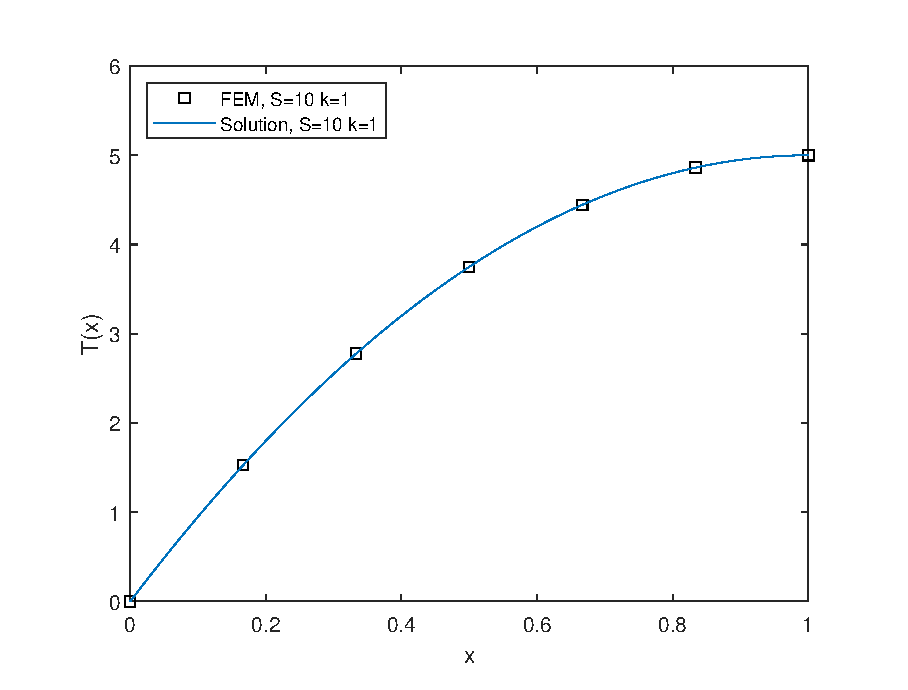
\includegraphics{./homework2/img/final_FEM.eps}
    \caption{Analytical Solution and FEM Approximation}
    \label{fig:sol_FEM}
\end{figure}
%\begin{figure}[htb!]
%    \centering
%    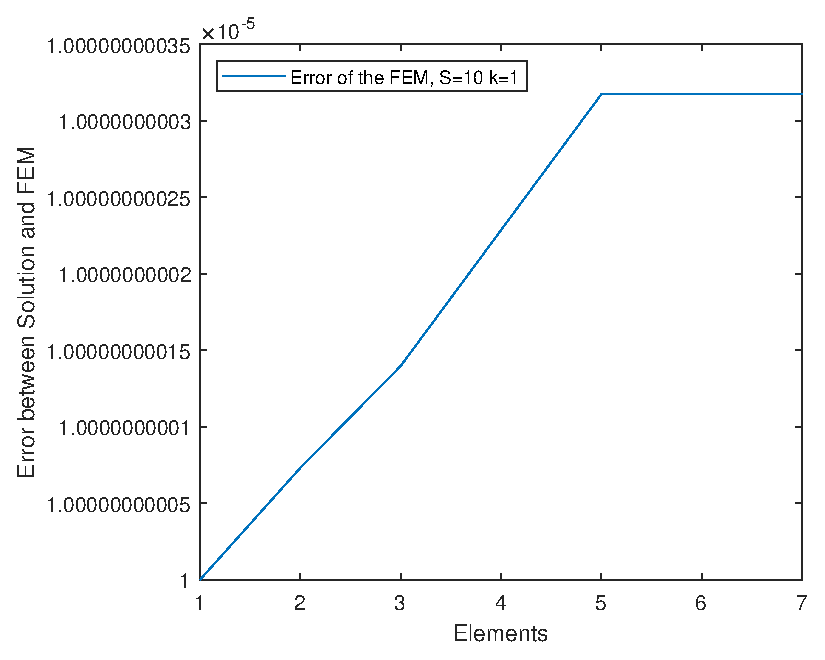
\includegraphics{./homework2/img/5.eps}
%    \caption{Absolute Error of the FEM}
%    \label{fig:error}
%\end{figure}
     \section*{Midterm Exam}
     \addcontentsline{toc}{section}{Midterm Exam}
     \subsection*{Q1}
\addcontentsline{toc}{subsection}{Q1} 
\begin{enumerate}[label=\alph*]
    \item In CT images it is easy to differentiate different types of soft tissues.
    \subitem False, soft tissues have a similar effective attenuation coefficient. Therefore, it is not easy to distinguish between soft tissues, but soft and hard tissue.
    \item There are no biological hazards due to x-ray exposure.
    \subitem False, due to the high energy of x-ray beams, which causes ionization of tissue, the biological risk is of a mutagenic resp. cancerogenic manner.
    \item The 2D Fourier transform of the image can be obtained from the acquired sinogram.
    \subitem True, the Fourier slice theorem specifies exactly this issue.
   % \begin{equation*}
%        \mu (x,y) = \frac{1}{4\pi^2}\int_{0}^{2 \pi} %{\int_{-\infty}^{+\infty}{\frac{1}{-x \sin{\theta} + y \cos{\theta} - s}\  %\frac{\partial R(\theta,s)}{\partial s}ds d\theta}}
%    \end{equation*}
    \item No representative images are rendered with back-projection when the views are not filtered.
    \subitem True, in order to enhance the contrast of features in the picture you have to filter it, though.
    \item The total attenuation of a non-monochromatic x-ray beam increases linearly with depth for a uniform medium.
    \subitem True,
    \begin{equation}
        \textbf{I} = I_0\ e^{-\mu_1 L_1} e^{-\mu_2 L_2} e^{-\mu_3 L_3} = I_0 e^{\underbrace{-\mu_1 L_1 -\mu_2 L_2- \mu_3 L_3}_{\text{\normalfont linear terms}}}
    \end{equation}    
\end{enumerate}

\subsection*{Q2}
\addcontentsline{toc}{subsection}{Q2} 
\subsubsection*{a}
\addcontentsline{toc}{subsubsection}{a} 
\begin{figure}[!htb]
    \centering
    \includegraphics[width=.4\linewidth]{./midterm/img/3.eps}
    \caption{Signal shape at 0\textdegree}
    \label{fig:0}
\end{figure}
\begin{figure}[!htb]
    \centering
    \includegraphics[width=.4\linewidth]{./midterm/img/1.eps}
    \caption{Signal shape at 45\textdegree}
    \label{fig:45}
\end{figure}
\begin{figure}[!htb]
    \centering
    \includegraphics[width=.4\linewidth]{./midterm/img/2.eps}
    \caption{Signal shape at 90\textdegree}
    \label{fig:90}
\end{figure}
\clearpage
\subsubsection*{b}
\addcontentsline{toc}{subsubsection}{b} 
As seen in the figures \ref{fig:0},\ref{fig:45} and \ref{fig:90}, the highest peak of the accumulated intensity is at the signal from 45\textdegree. The position of $2\sqrt{2}$ on the x-axis of plot \ref{fig:45} corresponds thereby to the complete diagonal ray from the lower left to the upper right corner in the lower scheme (Fig. \ref{fig:perfect_ray}).
\begin{figure}[!htb]
    \centering
    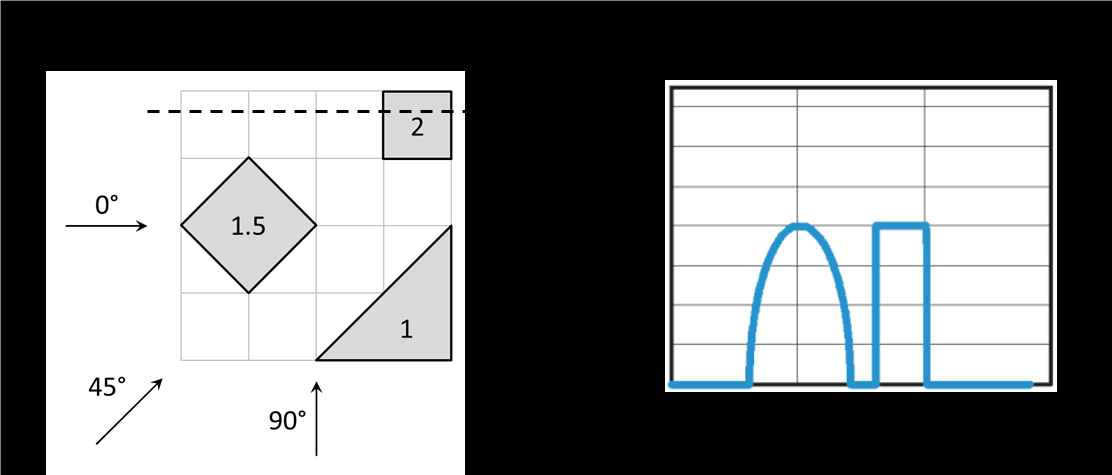
\includegraphics[clip,width=.6\linewidth,trim=9mm 0mm 115mm 13mm]{./midterm/img/Rays.png}
    \caption{Perfect Ray}
    \label{fig:perfect_ray}
\end{figure}



\subsection*{Q3}
\addcontentsline{toc}{subsection}{Q3} 
Calculate resolution of an optical microscope given the following characteristics:
\begin{itemize}
    \item Magnification $\textbf{M}$ = 60x
    \item Lens Diameter $\textbf{D}$ = \SI{9.4}{\milli\meter}
    \item Focal Length $\textbf{f}$ = \SI{2.4}{\mm}
    \item Immersion Medium: oil, $\textbf{n}$ = 1.33
    \item Illumination \boldmath$\lambda$ = \SI{560}{\nm}
\end{itemize}

\begin{align}
    d &= \frac{\lambda}{2 \mathrm{NA}} \\
    &= \frac{\lambda}{2 n \sin{\theta}} \\
    &= \frac{\lambda}{2 n \Big(\frac{0.5 D}{\sqrt{(0.5 D)^2 + f^2}}\Big)}\\
    &= \frac{\SI{560}{\nano\meter}}{2\ \cdot\ \num{1.33}\ \cdot\ \Big(\frac{0.5 \cdot \SI{9.4}{\mm}}{\sqrt{(0.5 \SI{9.4}{\mm})^2 + (\SI{2.9}{\mm}^2}}\Big)}\\
    &= \SI{0.25}{\micro\meter}
\end{align}

\subsection*{Q4}
\addcontentsline{toc}{subsection}{Q4} 
Which parameters influence the depth (slice thickness) that can be efficiently visualized by an optical microscope? How could high resolution images of thicker slices be obtained by a conventional microscope?
\\[2\baselineskip]
The main parameter to influence the penetration into the sample is the scattering inside. Furthermore, the wavelength and light intensity are also crucial physical parameters. At the optical microscope Numerical Aperture (resp. the diffraction), the optical density and reflectance of the sample influence imaging.\\
To overcome these hurdles an increase in NA resp. light intensity and/or a decrease in wavelength could yield more resolution. Generally speaking, the the overall diffraction limit (Abbe) has to be maxed out.


\subsection*{Q5}
\addcontentsline{toc}{subsection}{Q5} 
\begin{enumerate}[label=\alph*]
    \item The width of a signal in the time domain is proportional to the width in the frequency domain.
    \subitem True, the width in time domain is indirect proportional to a signal in the frequency domain. 
    \item The central pixel in the 2D k-space (k$_x$=0,k$_y$=0) corresponds to a uniform image in the space domain.
    \subitem True, the center of  the 2D k-space is a uniform image. One pixel corresponds to a constant picture frequency which means a uniform image in the space domain.
    \item A one-dimensional wave characterized by $u = u_0 \cos(−5x+3t−2.5)$ propagates towards the negative x direction.
    \subitem False, it propagates in the positive x-Direction (+3t Term)
    \item Deconvolution is particularly suited for systems with a narrow frequency response.
    \subitem True, a narrow frequency response implies that the image possesses only few strong gradients and therefore the image has poor feature edge quality. A deconvolution then sharpens the image.
    \item For a given aperture, diffraction is more prominent in the ultraviolet than in the infrared. 
    \subitem False, diffraction increases with increasing wavelength. The focal size of a microscope is ultimately diffraction limited and proportional to the wavelength.
    \begin{equation}
        d =\frac{\lambda}{2NA}
    \end{equation}
\end{enumerate}


\subsection*{Q6}
\addcontentsline{toc}{subsection}{Q6} 
For a diffuse medium with prominent Rayleigh scattering, provide the wavelength dependence of the effective attenuation coefficient in a spectral range where the absorption coefficient increases linearly with wavelength.\\
Effective Attenuation Coefficient:\\
\begin{align}
    \mu_{eff} &= \sqrt{\frac{\mu_a}{D}},\ \mathrm{with}\ D = \frac{1}{3(\mu_a + \mu_s(1-g)},\ \mathrm{with}\ g \in [0.65,0.95] \\
    &= \sqrt{\mu_a\ \cdot\ 3(\mu_a + \mu_s(1-g))}
\end{align}
According the diffusion approximation that can be applied to solve the RTE scattering events are dominant over the absorption $\mu_s \gg \mu_a$. We therefore neglect the additive $\mu_a$.\\
Furthermore, Rayleigh scattering effects are dominant over others, which simplifies the equation according to $\mu_s \propto \lambda^{-4}$. With the wavelength dependence of the absorption coefficient $\mu_a \propto \lambda$, this leads to:
\begin{align}
\mu_{eff} &= \sqrt{3\mu_a\mu_s(1-g)}\\
&= \sqrt{3\lambda\lambda^{-4}(1-g)}\\
\Rightarrow \mu_{eff} &\propto \lambda^{-3/2}
\end{align}

\subsection*{Q7}
\addcontentsline{toc}{subsection}{Q7} 
An ideal camera moves in the x direction with constant velocity $\nu$ during exposure. If the exposure time is $\nu$ derive an expression for the point spread function and the transfer function of the imaging system. Demonstrate the effect of such motion on an image of your choice, assuming that $\nu T$ = 10 pixels. Provide Matlab code.

The PSF can be computed by:
\begin{equation}
f(x,y) = \begin{cases} \frac{1}{v\ T_{end}}, &for\ 0 \leq x \leq v T_{end} \\ 0, &otherwise \end{cases}
\end{equation}
Then, the images are overlapped along the interval by tranlation of the original picture.
\begin{lstlisting}
vT = 10;
img_orig = importdata('lena_full.png');
img = img_orig/(vT+1);
for i = 1:vT
    img = img + imtranslate(img_orig/(vT+1),[i 0]);
end
figure;
imshow(img_orig);
figure;
imshow(img);
imwrite(img,'lena_blurry.png');
\end{lstlisting}

\begin{figure}[htb!]
\begin{subfigure}[c]{0.5\linewidth}
\centering
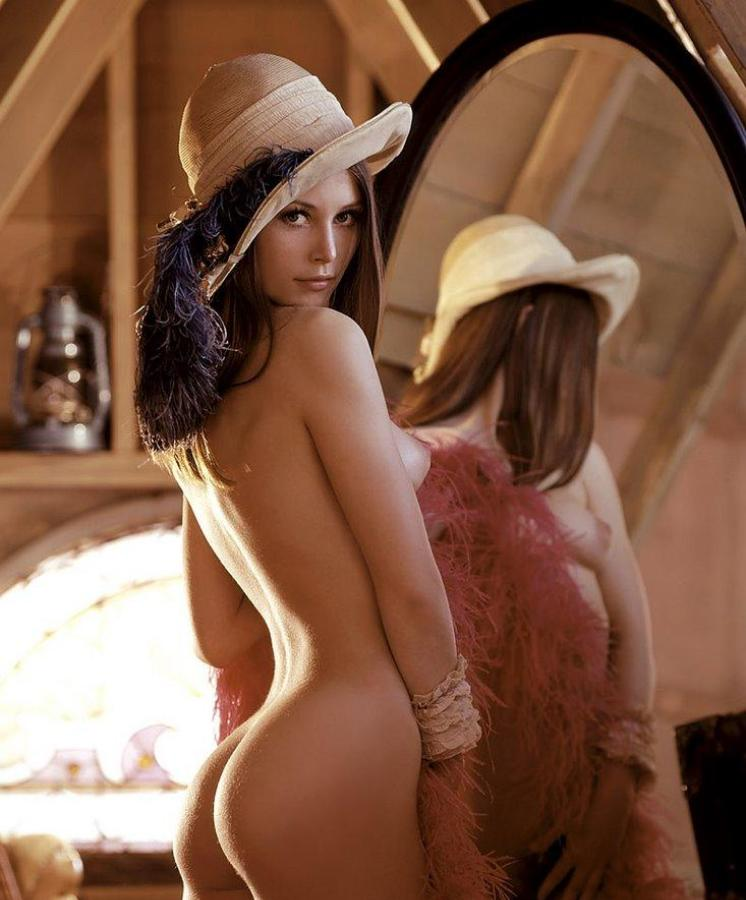
\includegraphics[clip, trim=0 0mm 0 0,width=0.8\linewidth]{./midterm/img/lena_full.png}
\subcaption{Original Figure}
\end{subfigure}
\begin{subfigure}[c]{0.5\linewidth}
\centering
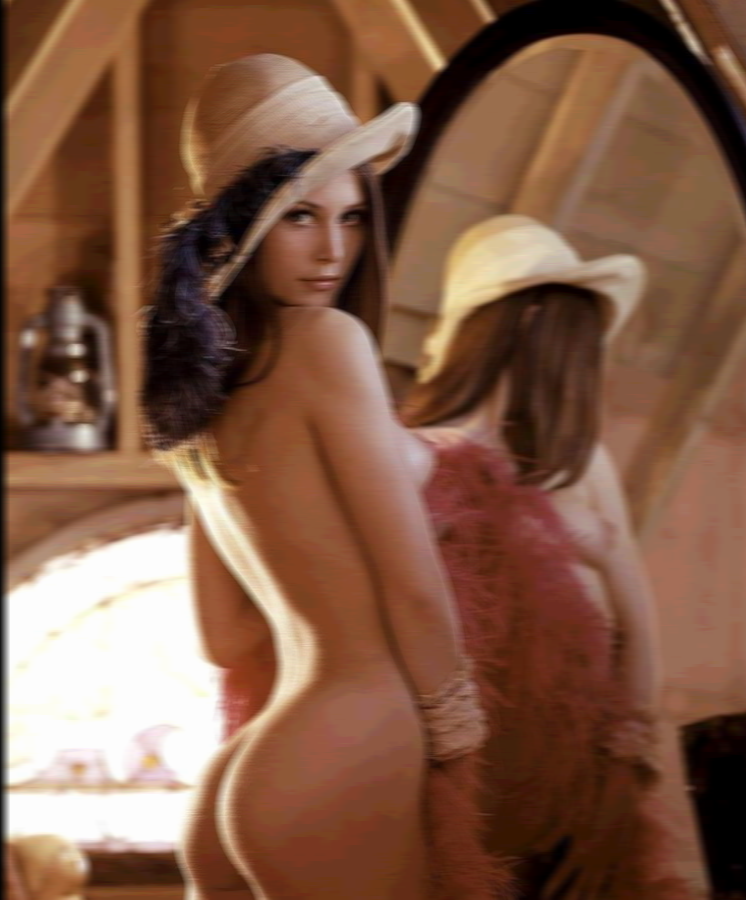
\includegraphics[clip, trim=0 0mm 0 0,width=0.8\linewidth]{./midterm/img/lena_blurry.png}
\subcaption{Blurry Picture}
\end{subfigure}

\caption{Pictures before and after processing}
\end{figure}

\subsection*{Q8}
\addcontentsline{toc}{subsection}{Q8} 
An infinitely large non absorbing medium with a high concentration of small spherical scatters is irradiated with blue, yellow and red light. Which beam penetrates deeper? Why? Give an analytical explanation.
\\[2\baselineskip]
As shown in the Planck-Einstein-Relation $E=h\frac{c}{\lambda}$, the light with low wavelength contains more energy than light with higher wavelengths. Therefore, photons with high energy scatter more often in tissue than photons with lower energy. Hence, even with anisotropic scattering high-energy photons pass more times the mean free path between to scattering events than low-energy photons.


\subsection*{Q9}
\addcontentsline{toc}{subsection}{Q9} 
Derive central, forward and backward finite difference approximations for the second order derivative $f''(x)$ of a function of one variable $f(x)$ ?
What is the truncation error of the derived approximations?\\
Forward Difference:\\
\begin{align}
    f'(x) &\approx \frac{f(x+h) -f(x)}{h}\\
    Then,\    f''(x) &\approx \frac{f'(x+h)-f'(x)}{h}\\
    &=\frac{\frac{f(x+2h)-f(x+h)}{h}-\frac{f(x+h)-f(x)}{h}}{h}\\
    &=\frac{f(x+2h)-2f(x+h)+f(x)}{h^2}
\end{align}
Truncation Error: $O(h)$\\
Backward Difference:\\
\begin{align}
    f'(x) &\approx \frac{f(x) -f(x+h)}{h}\\
    Then,\    f''(x) &\approx \frac{f'(x)-f'(x-h)}{h}\\
    &=\frac{\frac{f(x)-f(x-h)}{h}-\frac{f(x-h)-f(x-2h)}{h}}{h}\\
    &=\frac{f(x)-2f(x-h)+f(x-2h)}{h^2}
\end{align}
Truncation Error: $O(h)$\\

Central Difference:\\
\begin{align}
    f'(x) &\approx \frac{f(x+h) -f(x-h)}{2h}\\
    Then,\    f''(x) &\approx \frac{f'(x+2h)-f'(x-h)}{2h}\\
    &=\frac{\frac{f(x+2h)-f(x)}{2h}-\frac{f(x)-f(x-2h)}{h}}{2h}\\
    &=\frac{f(x+2h)-2f(x)+f(x-2h)}{4h^2}\\
    &\overset{h' = \frac{h}{2}}{=}\frac{f(x+h')-2f(x)+f(x-h')}{h'^2} \label{eq:2nd_central}
\end{align}
Truncation Error: $O(h^2)$



\subsection*{Q10}
\addcontentsline{toc}{subsection}{Q10} 
Using the central difference approximation, derive a coefficient matrix $\mathbf{A}$ corresponding to the following boundary problem:

\begin{align}
  f''(x) &=(1-x\sin{x}) f(x),\ x \in [0,2]\label{eq:2nd_base}\\
  f(0) &= \alpha\\
  f(2) &= \beta
\end{align}

with the equation \ref{eq:2nd_central} and \ref{eq:2nd_base} 
\begin{align}
(1-x\sin{x}) f(x) &= \frac{f(x+h)-2f(x)+f(x-h)}{h^2}\\
(1-x_{i} \sin(x_{i})) f(x_i) &\overset{x + h= x_{i+1}}{\underset{x - h= x_{i-1}}{=}} \frac{f(x_{i+1})-2f(x_i)+f(x_{i-1})}{h^2}\\
(2 + h^2-h^2x_{i} \sin(x_{i})) f(x_i) - f(x_{i+1}) - f(x_{i-1}) &= 0\\
\mathrm{Substitute}\ \xi\ &= (2 + h^2-h^2x_{i} \sin(x_{i}))\\
\begin{bmatrix}
\xi & -1 & 0  & ... & ... & ... & 0\\
-1 & \xi & -1  & 0& &  & \vdots\\
0 & -1 & \xi & -1& 0 & &  \vdots\\
\vdots & \vdots & \vdots& \vdots & \vdots& \vdots & \vdots\\
 \vdots & &  & 0 & -1 & \xi & -1\\
0 & ... & ... & ... & 0 & -1 & \xi
\end{bmatrix}\begin{bmatrix}
f_2 \\ f_3 \\ f_4 \\ \vdots\\f_{N-1}\\ f_N
\end{bmatrix}&= \begin{bmatrix}
\alpha \\ 0 \\ 0 \\ \vdots\\ 0 \\ \beta
\end{bmatrix}
\end{align}

     \section{Homework 3}
     \subsection{Assignment: Newton's Method}
This method is a standard way in mathematics to find zeros of a function numerically. Graphically speaking, one computes the zero-crossing point of a tangent to a point on the function itself in each iteration. The projection of the zero onto the function serves as the new starting point in the following iteration. In each step, the algorithm approximates the zero more precisely until the method is aborted below a certain error.
For the exercise, the starting point (\ref{eq:start}) for a function (\ref{eq:fun}) as well as the precision (\ref{eq:prec}) and its abortion criterion (\ref{eq:abortion_crit}) are given. In this case, we do not want to find the zeros of a provided function, but of its derivative in order to find the extremum. Therefore, substituting equation \ref{eq:newton} with $g(x) = f'(x)$ simplifies to eq. \ref{eq:newton'}.
\begin{align}
    x_0 &= 0.5 \label{eq:start}\\
    f(x)\ &=\ \frac{x}{2}\ -\ \sin(x)\label{eq:fun}\\
    \epsilon\ &=\ \num{1e-5} \label{eq:prec}\\
     x_{k+1} &= x_k - \frac{g(x_k)}{g'(x_k)}\label{eq:newton}\\
    x_{k+1} &= x_k - \frac{f'(x_k)}{f''(x_k)} \label{eq:newton'}\\
    \epsilon\ &>\ \mathopen|x_{k+1}\ -\ x_k\mathclose| \label{eq:abortion_crit}
\end{align}

To the specified maximal error, the algorithm converges in five steps. Figure \ref{fig:newton} shows the function, the starting points (grey) and the approximated zeros (red). The last iterations cannot be distinguished in the plot, because the approximating lies already close to the zero of the function. By inspection of the plot, we can validate that the found extremum is a minimum.
\clearpage
\begin{figure}[!htb]
    \centering
    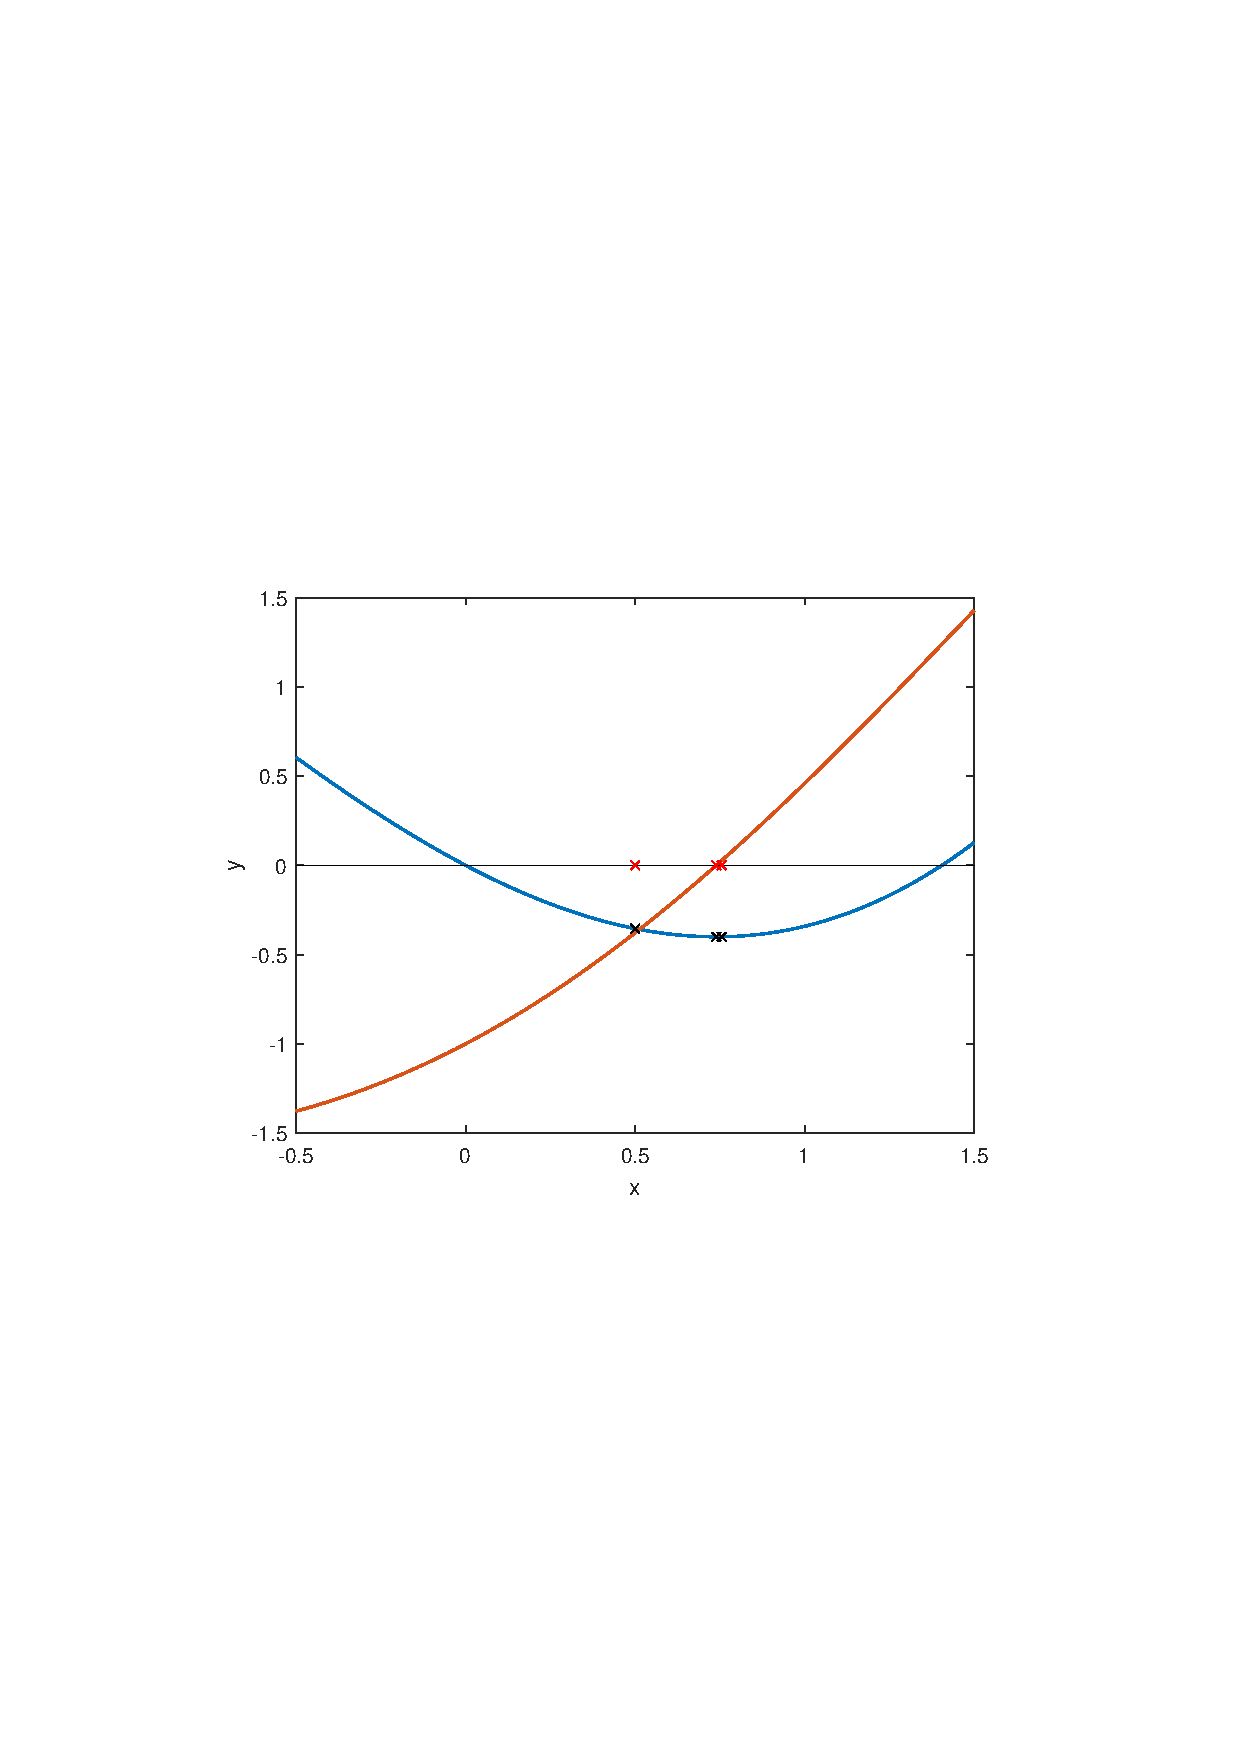
\includegraphics[trim={60 260 50 260},clip, width=.8\linewidth]{./homework3/img/NewtonMethod.pdf}
    \caption{Approximated zeros of a function by the Newton Method. The orange Graph depicts the derivative of the blue function (\ref{eq:fun}).}
    \label{fig:newton}
\end{figure}

\begin{lstlisting}
syms f(x)
f(x) =  ((x.^2)./2) - sin(x);
df = diff(f,x);
ddf = diff(df,x);
x_prev = 0.5;
e = 1;
iterations = 1;
x = -0.5:0.001:1.5;
figure;
plot(x,double(f(x)),'LineWidth',1.2,'DisplayName','f(x)');
hold on
plot(x,double(df(x)),'LineWidth',1.2,'DisplayName','f''(x)');
l = refline([0 0]);
l.Color = [0,0,0];
l.LineStyle = '-';
l.LineWidth = 0.1;
while e >= 1e-5
    x_next = x_prev - (double(df(x_prev))/double(ddf(x_prev)));
    e = abs(x_next - x_prev);  
    plot(x_prev,double(f(x_prev)),'kx');
    plot(x_prev,0,'rx');
    x_prev = x_next;
    iterations = iterations + 1;
end
xlabel('x');
ylabel('y');
print('fig/NewtonMethod.pdf','-dpdf');
\end{lstlisting}
     \subsection{Assignment: An imaging problem}
Consider the following imaging problem (see Fig. 1): 3 light emitters ($E_j,\ j\in [1,3]$) are
positioned in known locations in a room. In order to find the power emanating from the
emitters, 4 detectors ($D_i,\ i\in[1,4]$) are positioned at certain locations. The power $I_d$ measured by the $i$-th detector is given by:
\begin{align}
    I_{d,i}\ &=\ \sum_{j=0}^{N}\frac{I_{e,j}}{\mathopen|r_{ij}\mathclose|^2},\\
    r_{ij}\ &=\ \sqrt{(D_i\ -\ E_j)^2}\\
    \mathrm{Imaging\ Forward\ Problem: }\ \mathbf{A I_e} &= \mathbf{I_d}\\
    \mathrm{Imaging\ Inverse\ Problem: }\ \mathbf{I_e} &= \mathbf{A^{-1} I_d}\\  
\end{align}
where I$_{e,j}$ is the power of the $j$-th intensity source and r$_{ij}$ is the Distance between the detector and emitter.



\subsubsection{Build the matrix for the imaging problem defined above}
\begin{lstlisting}
%% Assignment 2 An imaging problem
% a
s.orig.D = [-1,1;1,1;1,-1;-1,-1];
s.orig.E = [-0.5,0.5;0,0;0.5,0.5];
s.orig.I_e = [4,3,1];
s.orig.A = zeros(length(s.orig.D),length(s.orig.E));

for i = 1:length(s.orig.D)
    for j = 1:length(s.orig.E)
        s.orig.A(i,j) = 1./sqrt(sum((s.orig.D(i,:)-s.orig.E(j,:)).^2));
    end
end
\end{lstlisting}




\subsubsection{What are the detected values for the source values [$\mathbf{I_{e,1}, I_{e,2}, I_{e,3}}$] = [$\mathbf{4, 3, 1}$]?
Consider these detected values as the measured data.}
\begin{lstlisting}
%% b
s.orig.I_d = s.orig.A * s.orig.I_e';
\end{lstlisting}

\begin{align}
\mathbf{A}\ &=\ \left(\begin{array}{ccc} \sqrt{2} & \frac{\sqrt{2}}{2} & \frac{\sqrt{2}\,\sqrt{5}}{5}\\ \frac{\sqrt{2}\,\sqrt{5}}{5} & \frac{\sqrt{2}}{2} & \sqrt{2}\\ \frac{\sqrt{2}}{3} & \frac{\sqrt{2}}{2} & \frac{\sqrt{2}\,\sqrt{5}}{5}\\ \frac{\sqrt{2}\,\sqrt{5}}{5} & \frac{\sqrt{2}}{2} & \frac{\sqrt{2}}{3} \end{array}\right)\\
\mathbf{I_d}\ &=\ \left(\begin{array}{c} 8.411\\ 6.065\\ 4.639\\ 5.123 \end{array}\right)
\end{align}




\clearpage
\subsubsection{Calculate the solution of the inverse problem based on the pseudo‐inverse of the
matrix}
\begin{lstlisting}
%% c
tol = 1e-5;
[s.orig.moore.I_e, s.orig.moore.A_inv] = SolPseudoInvMoore(s.orig.A,s.orig.I_d,tol);
\end{lstlisting}
\begin{lstlisting}
function [I_e_moore,A_inv_moore] = SolPseudoInvMoore(A,b,tol)
A_inv_moore = pinv(A,tol);
I_e_moore = A_inv_moore * b;
end
\end{lstlisting}
\begin{align}
    \mathbf{A_{inv,moore}}\ &=\ \left(\begin{array}{cccc} 1.144 & -0.08321 & -0.6567 & -0.4039\\ -0.8279 & -0.8279 & 1.535 & 1.535\\ -0.08321 & 1.144 & -0.4039 & -0.6567 \end{array}\right)\\
    \mathbf{I_{e,moore}}\ &=\ \left(\begin{array}{c} 4.0\\ 3.0\\ 1.0 \end{array}\right)
\end{align}



\clearpage
\subsubsection{ Calculate the solution of the inverse problem based on the singular value
decomposition (SVD) of the matrix}
\begin{align}
    \mathbf{A_{inv,SVD}}\ &=\ \left(\begin{array}{cccc} 1.144 & -0.08321 & -0.6567 & -0.4039\\ -0.8279 & -0.8279 & 1.535 & 1.535\\ -0.08321 & 1.144 & -0.4039 & -0.6567 \end{array}\right)\\
    \mathbf{I_{e,SVD}}\ &=\ \left(\begin{array}{c} 4.0\\ 3.0\\ 1.0 \end{array}\right)
\end{align}
\begin{lstlisting}
%% d
[s.orig.SVD.I_e, s.orig.SVD.A_inv] = SolPseudoInvSVD(s.orig.A,s.orig.I_d,0);
\end{lstlisting}
\begin{lstlisting}
function [I_e_SVD,A_inv_SVD] = SolPseudoInvSVD(A,b,truncate)
[U,S,V] = svd(A);

[m,n] = size(U);
U = U(1:m,1:n-truncate);

[m,n] = size(V);
V = V(1:m,1:n-truncate);

[m,n] = size(S);
S = S(1:m-truncate,1:n-truncate);

S_degger = S;
S_degger(S_degger > 0) = 1./S_degger(S_degger > 0);
A_inv_SVD = V * S_degger' * U';
I_e_SVD = A_inv_SVD * b;
end
\end{lstlisting}



\clearpage
\subsubsection{Calculate the solution of the inverse problem based on an iterative inversion
algorithm (lsqr)}

\begin{equation}
    \mathbf{I_{e,lsqr}}\ =\ \left(\begin{array}{c} 4.0\\ 3.0\\ 1.0 \end{array}\right)    
\end{equation}

\begin{lstlisting}
%% e
s.orig.LSQR.I_e = lsqr(s.orig.A,s.orig.I_d);
\end{lstlisting}



\clearpage
\subsubsection{Repeat steps c‐d when noise is added to the measurements. Compare the results
obtained by changing the locations of the detectors. Comment on the conditioning of
the problem.}
Noise with an amplitude of 1\% around actual value was added to the detection.\\
After moving the detectors three time the distance away from the sources, the error does not influence the third digit, but also the second and first after the point.\\
The posed problem is \textbf{well-posed}, because the three necessary conditions are satisfied:
\begin{enumerate}
    \item Existence $rank(A) = rank(A|I_{d,noise}) = 3$
    \item Uniqueness $rank(A) = size(A,2) = 3$
    \item Stability $pinv(A)*A = \mathbf{I}$
\end{enumerate}
 The conditions number of MATLAB's intrinsic \textit{cond()} then computes for the original A to \num{7.7272} and for the moved detectors to \num{25.01}. These numbers are both larger than 1, which shows, that the matrix inversion is sensitive to small changes before the inversion. Terefore we call both matrices \textbf{ill-conditioned}.
\begin{align}
\mathbf{A_{inv,moore,noise}}\ &=\ \left(\begin{array}{cccc} 1.144 & -0.08321 & -0.6567 & -0.4039\\ -0.8279 & -0.8279 & 1.535 & 1.535\\ -0.08321 & 1.144 & -0.4039 & -0.6567 \end{array}\right)\\
\mathbf{I_{e,moore,noise}}\ &=\ \left(\begin{array}{c} 3.998\\ 3.0\\ 0.9992 \end{array}\right)\\
\mathbf{A_{inv,SVD,noise}}\ &=\ \left(\begin{array}{cccc} 1.144 & -0.08321 & -0.6567 & -0.4039\\ -0.8279 & -0.8279 & 1.535 & 1.535\\ -0.08321 & 1.144 & -0.4039 & -0.6567 \end{array}\right)\\
\mathbf{I_{e,SVD,noise}}\ &=\ \left(\begin{array}{c} 3.998\\ 3.0\\ 0.9992 \end{array}\right)
\end{align}

Detectors moved 3-times farer away:
\begin{align}
\mathbf{I_{e,moore,noise}}\ &=\ \left(\begin{array}{c} 4.041\\ 2.836\\ 1.122 \end{array}\right)\\
\mathbf{I_{e,SVD,noise}}\ &=\ \left(\begin{array}{c} 3.901\\ 2.976\\ 1.121 \end{array}\right)
\end{align}

\begin{lstlisting}
%% f
interval = [-0.1,0.1];
noise = interval(1) + (interval(2) - interval(1)) * rand(length(s.orig.I_d),1);
s.noise.I_d = s.orig.I_d + noise;
[s.noise.moore.I_e,s.noise.moore.A_inv] = SolPseudoInvMoore(s.orig.A,s.noise.I_d,tol);
[s.noise.SVD.I_e, s.noise.SVD.A_inv] = SolPseudoInvSVD(s.orig.A,s.noise.I_d,0);
% Compare Results with detectors manifold times farer away
factor = 3;
s.orig.moved.D = s.orig.D * factor;
for i = 1:length(s.orig.D)
    for j = 1:length(s.orig.E)
        s.orig.moved.A(i,j) = 1./sqrt(sum((s.orig.moved.D(i,:)-s.orig.E(j,:)).^2));
    end
end
s.noise.moved.I_d = (s.orig.moved.A * s.orig.I_e') + noise;
[s.noise.moved.moore.I_e,s.noise.moved.moore.A_inv] = ...
    SolPseudoInvMoore(s.orig.moved.A,s.noise.moved.I_d,tol);
[s.noise.moved.SVD.I_e, s.noise.moved.SVD.A_inv] = ...
    SolPseudoInvSVD(s.orig.moved.A,s.noise.moved.I_d,0);
% Conditioning
cond_num = cond(s.orig.A); %7.7273 --> ill-conditioned
cond_num_hat = cond(s.orig.moved.A); % 25.01 --> ill-conditioned
\end{lstlisting}





\clearpage
\subsubsection{Add 2 other sources ($\mathbf{E_4}$ and $\mathbf{E_5}$) close to $\mathbf{E_3}$ in the problem above.}
\begin{equation}
\mathbf{A}\ =\ \left(\begin{array}{ccccc} 1.414 & 0.7071 & 0.6325 & 0.6063 & 0.6565\\ 0.6325 & 0.7071 & 1.414 & 1.768 & 1.179\\ 0.4714 & 0.7071 & 0.6325 & 0.6063 & 0.6565\\ 0.6325 & 0.7071 & 0.4714 & 0.4419 & 0.5051 \end{array}\right) 
\end{equation}

\begin{lstlisting}
%% g
distance = [0.1, 0.1];
s.orig.added.E = [s.orig.E;s.orig.E(3,:) + distance;s.orig.E(3,:) - distance];
for i = 1:length(s.orig.D)
    for j = 1:length(s.orig.added.E)
        s.orig.added.A(i,j) = 1./sqrt(sum((s.orig.D(i,:)-s.orig.added.E(j,:)).^2));
    end
end
\end{lstlisting}




\clearpage
\subsubsection{Calculate the solution of the inverse problem with and without adding noise. Assume
source values of  [$\mathbf{I_{e,1}, I_{e,2}, I_{e,3},I_{e,4},I_{e,5}}$] = [$\mathbf{4, 3, 1, 1, 1}$]}

\begin{align}
\mathbf{I_{e,noise}}\ &=\ \left(\begin{array}{c} 4.003\\ 2.992\\ 0.9956\\ 1.001\\ 1.009 \end{array}\right)\\
   \mathbf{I_d}\ &=\ \left(\begin{array}{c} 9.674\\ 9.012\\ 5.902\\ 6.07 \end{array}\right)\\
   \mathbf{I_{d,noise}}\ &=\ \left(\begin{array}{c} 9.675\\ 9.014\\ 5.902\\ 6.068 \end{array}\right)
\end{align}
\begin{lstlisting}
%% h
s.orig.added.I_e = [s.orig.I_e'; 1; 1];
s.orig.added.I_d = s.orig.added.A * s.orig.added.I_e;
noise = interval(1) + (interval(2) - interval(1)) * rand(length(s.orig.added.I_e),1);
s.noise.added.I_e = s.orig.added.I_e + noise;
s.noise.added.I_d = s.orig.added.A * s.noise.added.I_e;
\end{lstlisting}




\clearpage
\subsubsection{For the problem in g, perform the inversion with standard SVD and truncated SVD for
different levels of noise. Comment on the results.}
\begin{table}[htb!]
\centering
\begin{tabular}{|c|c|c|}
\hline
&Truncation: 0&\\
\hline
Noise:0\% & Noise:100\% & Noise: 1000\% \\
   \hline
I_{e}\ =\ \left(\begin{array}{c} 4.0\\ 2.998\\ 0.9516\\ 1.018\\ 1.031 \end{array}\right)       & 
 I_{e}\ =\ \left(\begin{array}{c} 4.026\\ 2.92\\ 0.9775\\ 1.001\\ 1.077 \end{array}\right) &
I_{e}\ =\ \left(\begin{array}{c} 4.265\\ 2.218\\ 1.211\\ 0.8445\\ 1.49 \end{array}\right)  \\
\hline
   \hline
&Truncation: 1&\\
   \hline
Noise:0\% & Noise:100\% & Noise: 1000\% \\
   \hline
I_{e}\ =\ \left(\begin{array}{c} 3.979\\ 2.692\\ 1.169\\ 0.5941\\ 1.598 \end{array}\right)      & 
 I_{e}\ =\ \left(\begin{array}{c} 4.008\\ 2.643\\ 1.174\\ 0.6178\\ 1.589 \end{array}\right)&
I_{e}\ =\ \left(\begin{array}{c} 4.264\\ 2.209\\ 1.218\\ 0.8317\\ 1.507 \end{array}\right)  \\
\hline
   \hline
&Truncation: 2&\\
   \hline
Noise:0\% & Noise:100\% & Noise: 1000\% \\
   \hline
I_{e}\ =\ \left(\begin{array}{c} 4.149\\ 2.403\\ 1.179\\ 0.7079\\ 1.53 \end{array}\right)       & 
 I_{e}\ =\ \left(\begin{array}{c} 4.149\\ 2.404\\ 1.182\\ 0.7123\\ 1.533 \end{array}\right) &
I_{e}\ =\ \left(\begin{array}{c} 4.144\\ 2.413\\ 1.211\\ 0.7512\\ 1.555 \end{array}\right)  \\
\hline
\end{tabular}
\caption{Different solutions of the inverse problem, with different margins of truncation for the SVD matrices and different levels of noise. Noise levels are computed relative to the noise level used in the exercises before.}
\end{table}

\begin{lstlisting}
%% i
s.orig.added.SVD.truncation = 0:1:2;
s.noise.added.SVD.I_e = cell(1,length(s.orig.added.SVD.truncation));
s.noise.added.SVD.A = cell(1,length(s.orig.added.SVD.truncation));

Level = noise*[0,1,10];

for i = s.orig.added.SVD.truncation
    for j = 1:size(Level,2)
     s.noise.added.SVD.I_d = s.orig.added.A * (s.orig.added.I_e + Level(:,j));
  [s.noise.added.SVD.I_e{i+1},s.noise.added.SVD.A{i+1}] = SolPseudoInvSVD(s.orig.added.A,s.noise.added.SVD.I_d,i);  
    digits(4);
    sprintf('Truncation:%d, Noise Level:%d\n',i,Level(1,j)./noise(1))
    latex(vpa(sym(s.noise.added.SVD.I_e{i+1})))
    end
end
\end{lstlisting}

\clearpage
\subsubsection{For the problem in g, compute the solution using Tikhonov regularization. Using Lcurve, determine an optimal regularization parameter in range [$\mathbf{10^{-4}; 10^{-4}\cdot2^{14}}$]
(simply double your regularization parameter every iteration). Show your L-curve,
explain its meaning and how the optimal regularization parameter was selected.}
An L-curve shows the behavior of the approximation error to the norm of the augmented regularization matrix $L$ (Numerical stability of method). By choosing the regularization parameter $\lambda$ in the corner of this graph, we can obtain a suffictient small numerical error and simultaneously minimize the numerical instabilities.

\begin{align}
\mathbf{L}\ &=\ \left(\begin{array}{ccccc} 0.9595 & -0.9144 & -0.5103 & 0.2028 & -0.6406\\ 0.2704 & 1.692 & -1.536 & -0.7097 & -1.102\\ -0.6313 & -0.03136 & 1.313 & -0.3647 & -0.2856\\ 0.5552 & 0.2245 & -0.1433 & 1.574 & 0.107\\ -0.4948 & -0.1816 & -0.09867 & 0.2989 & 1.471 \end{array}\right)\\
\lambda\ &=\ 0.071194016876375\\
\mathbf{q(\lambda)}\ &=\ \left(\begin{array}{c} 4.004\\ 2.293\\ 2.556\\ -0.6331\\ 1.895 \end{array}\right)
\end{align}

\begin{figure}[h!]
    \centering
    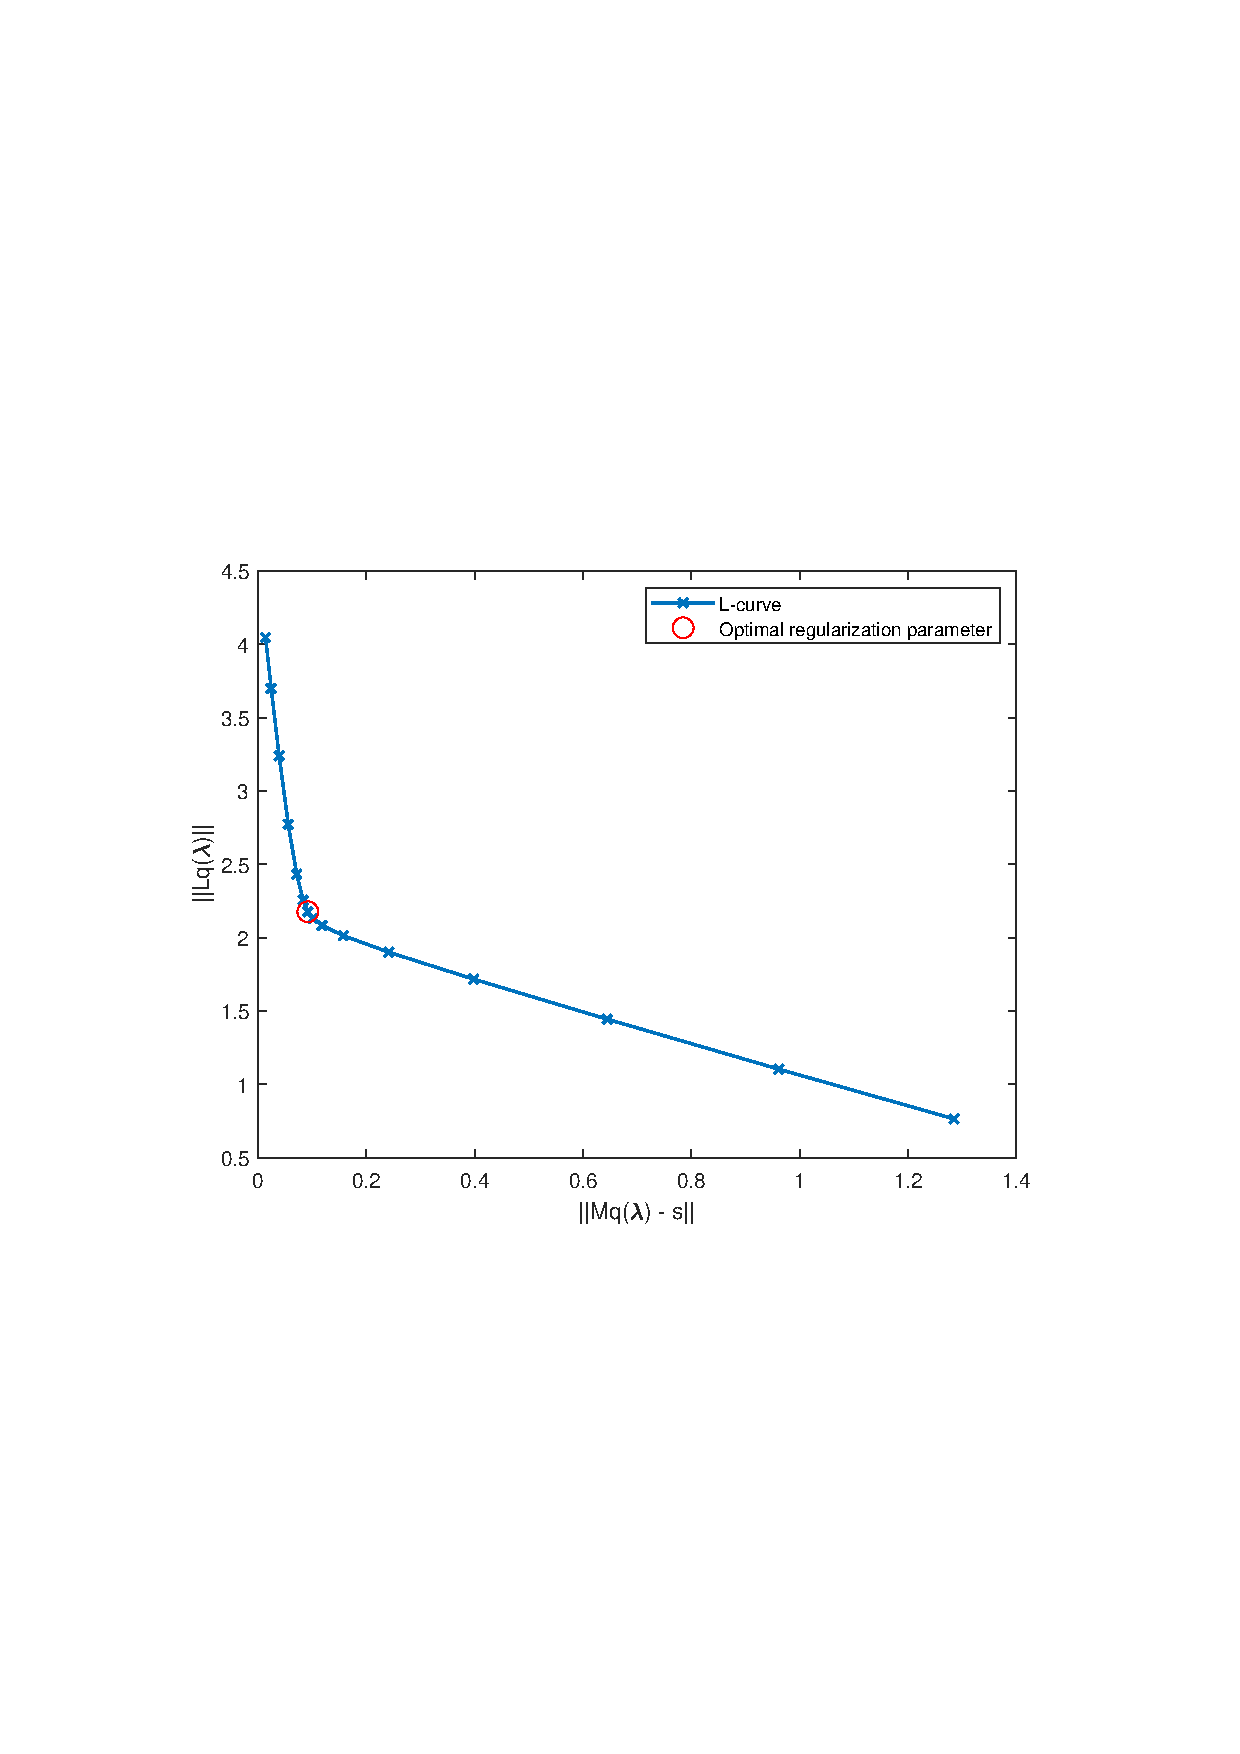
\includegraphics[trim={50 270 100 270},clip]{img/Tikhonov_real.pdf}
    \caption{Typical L-curve scheme with the smallest possible lambda with the most stable value.}
    \label{fig:tikh}
\end{figure}

\begin{lstlisting}
%% Tikhonov Regularization
M = s.orig.added.A;
s_tik = s.noise.added.I_d;
range = 1e-4 * 2.^(0:1:14);
x = zeros(length(range));
y = zeros(length(range));
L = eye(5) + 0.5*randn(5);
q_lam = @(lam) (M'*M+lam*(L'*L))\M'*s_tik;
mq_norm = @(lam) norm(M*q_lam(lam)-s_tik,2);
lq_norm = @(lam) norm(L*q_lam(lam),2);
q_norm = @(lam) norm(q_lam(lam),2);
x = arrayfun(mq_norm,range);
y = arrayfun(lq_norm,range);
dy = [0,diff(y)];
ddy = [0, diff(dy)];
dddy = [0, diff(ddy)];
max_dist = max(dddy);
fig =figure;
plot(x,y,'x-','LineWidth',1.2,'DisplayName','L-curve');
hold on
legend;
xlabel('||Mq(\lambda) - s||');
ylabel('||Lq(\lambda)||');
pos_opt = find(max(dddy)== dddy)+2;
plot(x(pos_opt),y(pos_opt),'ro','MarkerSize',10,'DisplayName',...
'Optimal regularization parameter');
q_lam(x(pos_opt))
print(fig,'fig/Tikhonov.eps','-dpdf');
\end{lstlisting}



    \section{Homework 4}
    \subsection{Bloch's Equation}
The pulse sequence diagram of an inversion-recovery spin echo sequence is given below.
The sequence is composed of a $\pi_y$ pulse, a $-\frac{\pi}{2}_y$ pulse and a $\pi_x$ pulse and it uses the
following parameters $TE$ = \SI{40}{\milli\s}, $TI$ = \SI{300}{\milli\s} and $TR$ = \SI{1500}{\milli\s}. The sequence is
employed to image a tissue with $T_1$ = \SI{1000}{\milli\s} and $T_2$ = \SI{80}{\milli\s}.
\begin{figure}[h!]
    \centering
    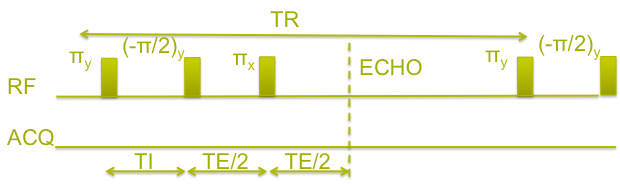
\includegraphics{./homework4/img/pulse_sequence.png}
    \caption{}
    \label{fig:my_label}
\end{figure}




\subsubsection{Consider a spin that precesses with off-resonance frequency equal to 1 Hz. Plot the
evolution of the angle of the transverse magnetization for the above spin for the $\mathbf{2^{nd}}$ $TR$.
Show that the spin echo is formed at time $TE$ from the $\mathbf{-\frac{\pi}{2}_y}$ RF pulse.}

\begin{figure}[h!]
\centering
    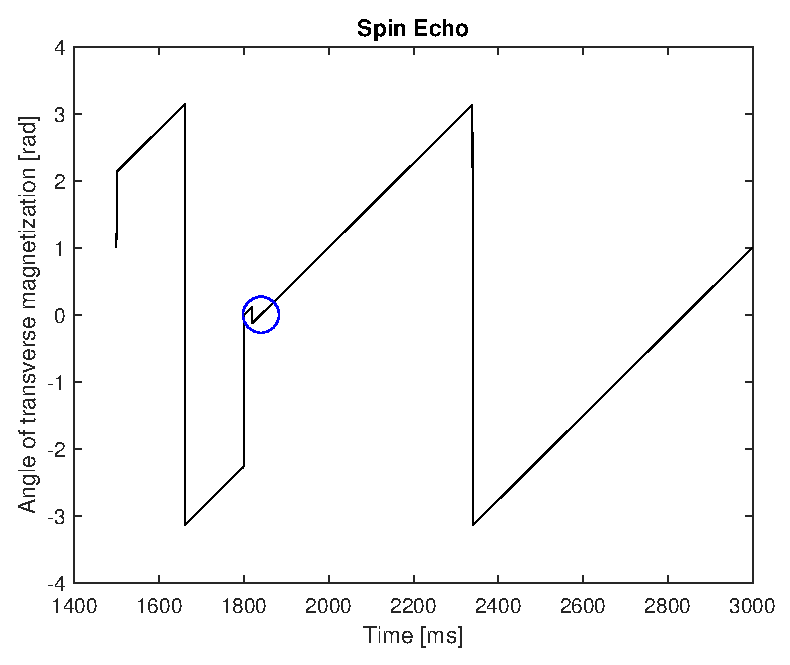
\includegraphics[width=\linewidth]{./homework4/img/Spin_Echo.eps}
    \caption{A spin echo is formed at $T_{echo} = TR\ +\ TI\ +\ TE\ =\ 1840\ ms$ (red circle).}
    \label{fig:spin_echo}
\end{figure}


\begin{lstlisting}
%% Assignment 1:
close all;
clear all;
df = 1; % Hz off-resonance.
T1 = 1000; % ms.
T2 = 80; % ms.
TE = 40; % ms.
TR = 1500; % ms.
TI = 300; % ms.
flip1 = pi; % pi y pulse
flip2 = -pi/2;% -pi/2 y pulse
flip3 = pi; % pi x pulse
dT = 1;
N_tr = round(TR/dT);
N_ti = round(TI/dT);
N_te = round(TE/dT);
N_tehalf = round(TE/(2*dT));
N_ex = 5; % number of RF excitations.
% magnetization vector
M=zeros(3,N_ex*N_tr);
% initial magnetization
M(:,1) = [0;0;1];
% Bloch equation matrices
R_flip1 = yrot(flip1);
R_flip2 = yrot(flip2);
R_flip3 = xrot(flip3);
[A1,B1] = freeprecess(dT,T1,T2,df);
% simulate Bloch equations
M_count=1;
% simulate Nex TRs
for n=1:N_ex
% pi RF excitation
M(:,M_count) = R_flip1*M(:,M_count);
% free-precession and relaxation over period TI
for k=1:N_ti
M_count=M_count+1;
M(:,M_count)=A1*M(:,M_count-1)+B1;
end
% pi/2 RF excitation
M(:,M_count) = R_flip2*M(:,M_count);
% free-precession and relaxation over period TR-TI
for k=1:N_tehalf
M_count=M_count+1;
M(:,M_count)=A1*M(:,M_count-1)+B1;
end
% pi RF excitation
M(:,M_count) = R_flip3*M(:,M_count);
% free-precession and relaxation over period TR-TI-TE/2
for k=1:(N_tr-N_ti-N_tehalf)

M_count=M_count+1;
M(:,M_count)=A1*M(:,M_count-1)+B1;
end
end
time = [0:M_count-1]*dT;
%% verify formation of echo by plotting angle of transverse magnetization
% for second TR
M_trans=M(1,:)+j*M(2,:);
figure;
plot(time(N_tr:2*N_tr),angle(M_trans(N_tr:2*N_tr)),'k-');
hold on;
scatter(N_tr+TI+TE,angle(M_trans(N_tr+TI+TE+1)), 300, 'b');
xlabel('Time [ms]');
ylabel('Angle of transverse magnetization [rad]');
title('Spin Echo');
print('img/Spin_Echo.eps','-depsc');
\end{lstlisting}

\subsubsection{Plot the evolution of longitudinal and transverse magnetization for 5 TRs. How many
TRs are required in order to establish a steady-state in the magnetization evolution?}
The stead state in the magnetization evolution is reached after $2\ TR$. (Fig. \ref{fig:inv_rec})
\begin{figure}[h!]
\centering
    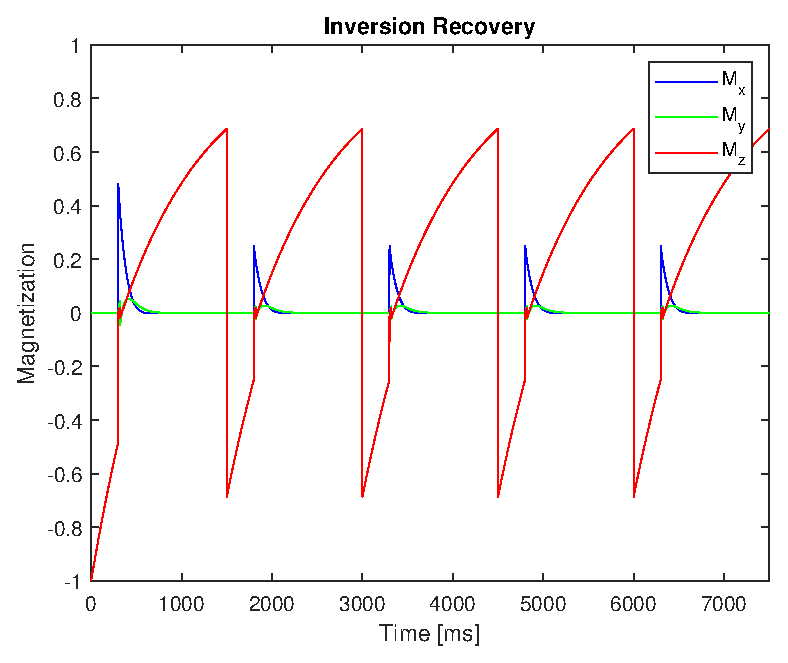
\includegraphics[width=\linewidth]{./homework4/img/Inversion_Recovery.eps}
    \caption{Inversion Recovery splitted into trajectories of the three cartesian field components.}
    \label{fig:inv_rec}
\end{figure}



\begin{lstlisting}
%% plot magnetization evolution
figure;
time = [0:M_count-1]*dT;
plot(time,M(1,:),'b-',time,M(2,:),'g-',time,M(3,:),'r-');
legend('M_x','M_y','M_z');
xlabel('Time [ms]');
ylabel('Magnetization');
axis([min(time) max(time) -1 1]);
title('Inversion Recovery');
print('img/Inversion_Recovery.eps','-depsc');
\end{lstlisting}


\subsubsection{Based on the numerical simulation of the Bloch equation, determine the signal of the
spin echo at the $\mathbf{5^{th}}$ TR (assume $\mathbf{M_0=1}$). Compare the signal of the formed spin-echo at the
$\mathbf{5^{th}}$ TR to the following analytical expression (depending on $\mathbf{T_1}$ and $\mathbf{T_2}$ relaxation times):}
The error between simulated and analytical solution is in the $3^{rd}$ digit. Hence, the simulation shows an accurate approximation.
\begin{align}
S\ &=\ M_0\left( 1-2e^{-\frac{TI}{T_1}}\ +\ 2e^{-\frac{TR-\frac{TE}{2}}{T_1}}\ -\ e^{-\frac{TR}{T_1}}\right)\ \cdot\ e^{-\frac{TE}{T_2}}\\
M_{echo,\ 5^{th}TR_x}\ &=\ 0.1532\\
M_{analytical,\ x}\ &=\ 0.1568
\end{align}

\begin{lstlisting}
%% signal at TE of the 5th TR based on numerical Bloch equation simulation
M_echo_5thTR = abs(M(:,4*N_tr+ N_ti + N_te));
M_echo_5thTR_x = M_echo_5thTR(1, :)
% signal based on analytical formula
M_analytical_x = abs((exp(-TE/T2))*(1-2*exp(-TI/T1)+exp(-TR/T1)))
\end{lstlisting}

\subsubsection{The above equation can be simplified for $\mathbf{TE<<TR}$:
Based on the analytic above expression, it is possible for a given TR to select the inversion time TI to null the signal of a tissue with a given $\mathbf{T_1}$. Assume that the inversion recovery spin echo sequence will be used to null the signal from fat ($\mathbf{T_1}$=360 ms). Find the inversion time required to null the fat signal.}
\begin{align}
S\ &=\ M_0\left( 1-2e^{-\frac{TI}{T_1}}\ +\ 2e^{-\frac{TR-\frac{TE}{2}}{T_1}}\ -\ e^{-\frac{TR}{T_1}}\right)\ \cdot\ e^{-\frac{TE}{T_2}}\\
S\ &\overset{TE<<TR}=\ M_0\ \left(1-2e^{-\frac{TI}{T_1}} + e^{-\frac{TR}{T_1}} \right) e^{-\frac{TE}{T_2}}\\
S\ &\overset{!}=\ 0,\  T_1(fat)\ =\ \SI{360}{\ms}\ \wedge\  TR\ =\ \SI{150}{\ms}\\
TI\ &=\ -T_1\ \mathrm{ln}\left(0.5\ +\ 0.5e^{-\frac{TR}{T_1}}\right)\\
TI\ &=\ -\SI{360}{\ms}\ \cdot\ \mathrm{ln}\left(0.5\ +\ 0.5e^{-\frac{\SI{150}{\ms}}{\SI{360}{\ms}}}\right)\ =\ \SI{243.94}{\ms}\\
TI_{sim}\ &=\ \SI{243.94}{\ms}
\end{align}

\begin{lstlisting}
T1fat=360; %ms
TR=1500; %ms
TI=-T1fat*log(.5+.5*exp(-TR/T1fat))
S=(1-2*exp(-TI/T1fat) + exp(-TR/T1fat))
\end{lstlisting}
    \subsection{Reconstruction from k-space}
The k-space data of a $T_1$-weighted sagittal brain image can be loaded from the workspace
braint1data.mat.


\subsubsection{Reconstruct the brain image using the given complex k-space data. Is it possible to
reconstruct the MR image using only the magnitude or the phase of the measured k-space
data? Show the corresponding images.}
A reconstruction with just the phase or magnitude information is not possible. Reducing one whole dimension causes too much information loss!
\begin{figure}[h!]
    \centering
    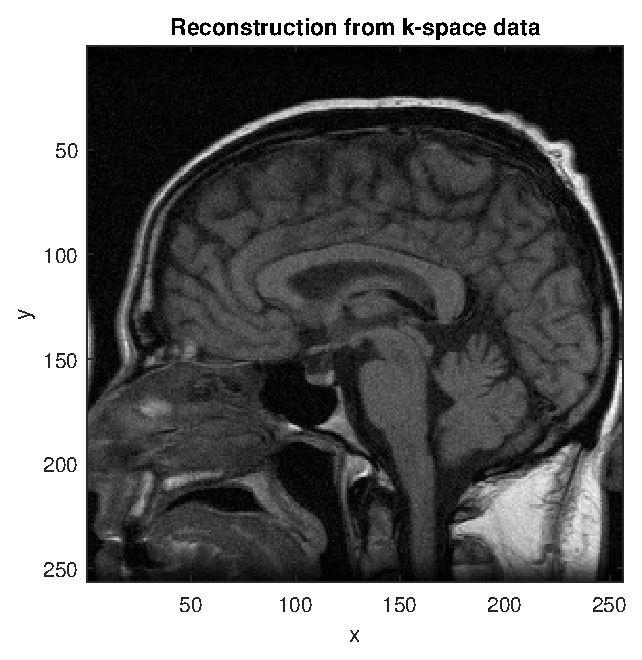
\includegraphics[width=.8\linewidth]{./homework4/img/recon.eps}
    \caption{Fully reconstructed image}
    \label{fig:recon}
\end{figure}

\begin{figure}[h!]
    \centering
    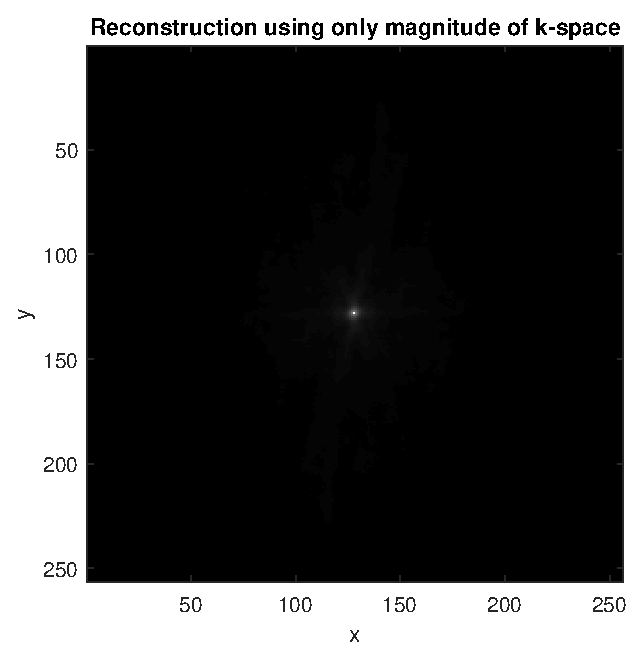
\includegraphics[width=.8\linewidth]{./homework4/img/recon_mag.eps}
    \caption{Reconstructed image without phase information}
    \label{fig:recon_mag}
\end{figure}

\begin{figure}[h!]
    \centering
    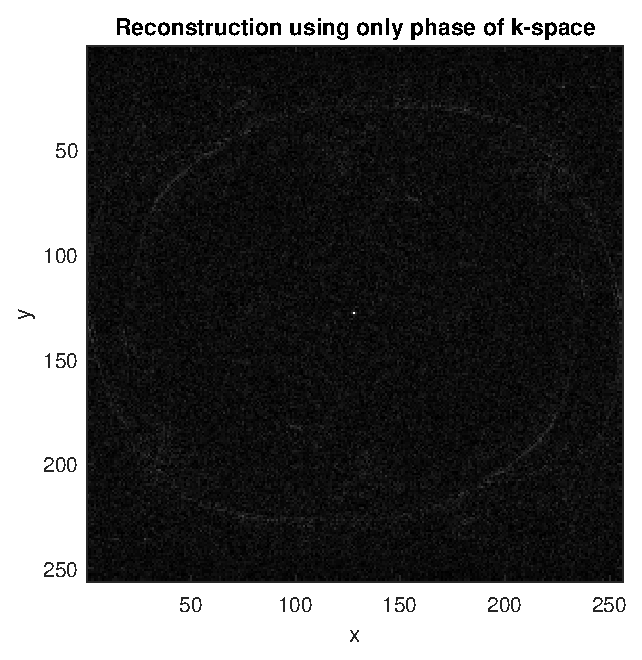
\includegraphics[width=.8\linewidth]{./homework4/img/recon_phase.eps}
    \caption{Reconstructed image without magnitude information}
    \label{fig:recon_phase}
\end{figure}
\clearpage

\begin{lstlisting}
%% reconstruct image using complex k-space data
img = ifft2c(rawkspace);
figure;
imagesc(abs(img));
colormap(gray);
axis equal tight;
title('Reconstruction from k-space data');
xlabel('x');
ylabel('y');
print('img/recon.eps','-depsc');
% using only magnitude of k-space
img = ifft2c(abs(rawkspace));
figure;
imagesc(abs(img));
colormap(gray);
axis equal tight;
title('Reconstruction using only magnitude of k-space');
xlabel('x');
ylabel('y');
print('img/recon_mag.eps','-depsc');
% using only phase of k-space
img = ifft2c(angle(rawkspace));
figure;
imagesc(abs(img));
colormap(gray);
axis equal tight;
title('Reconstruction using only phase of k-space');
xlabel('x');
ylabel('y');
print('img/recon_phase.eps','-depsc');
\end{lstlisting}



\subsubsection{Assume that only every other k-space point along the horizontal direction has been sampled. Reconstruct the MR image. What type of artifacts do you observe? Why?}

Sampling every second column causes a insufficient spacing in the k-space frquencies and therefore "orders" of the image. With large space between these, the higher orders will not be separated and overlap the central image. The overlap of the +1 and -1 "diffracted" order (in the Fourier space) with the central image (zeroth order) is cause of the "wrap". This effect is called aliasing in image processing.


\begin{figure}[h!]
    \centering
    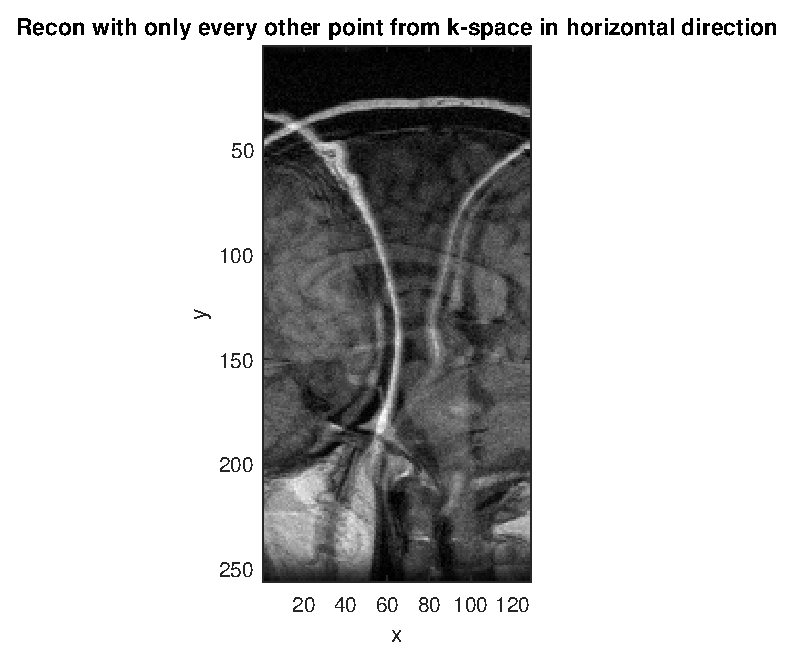
\includegraphics[width=.8\linewidth] {./homework4/img/recon_every2nd.eps}
    \caption{Reconstructed image with every other column in the k-space matrix.}
    \label{fig:recon_phase}
\end{figure}




\begin{lstlisting}
%% remove every other data point from k-space along x-axis
reduced_rawkspace = rawkspace;
reduced_rawkspace(:,1:2:end)=[];
%reconstruct image from reduced k-space data
reduced_ima = ifft2c(reduced_rawkspace);
figure;
imagesc(abs(reduced_ima));
colormap(gray);axis equal tight;
title(['Recon with only every other point from k-space' ...
' in horizontal direction']);
xlabel('x');
ylabel('y');
print('img/recon_every2nd.eps','-depsc');
\end{lstlisting}




\subsubsection{Raw k-space can be corrupted with noisy spikes of various origins. Introduce a spike
artifact in k-space, by setting the complex signal at the pixel location (160,160) equal to $10^4$. Reconstruct the MR image. How do k-space spike artifacts appear in image space?}


$\frac{160}{256} \cdot 360 = 180 + 45 $ -> information from a 225\textdegree angle in the image get superimposed. Normalization of the image with the highest magnitude squeezes the intensities of the k-space pixels togeher. Thus, it unitizes the reconstructed image's brightness. (What can be oberserved in increasing the pixels intensity to $10^5$ or higher) 

\begin{figure}[h!]
    \centering
    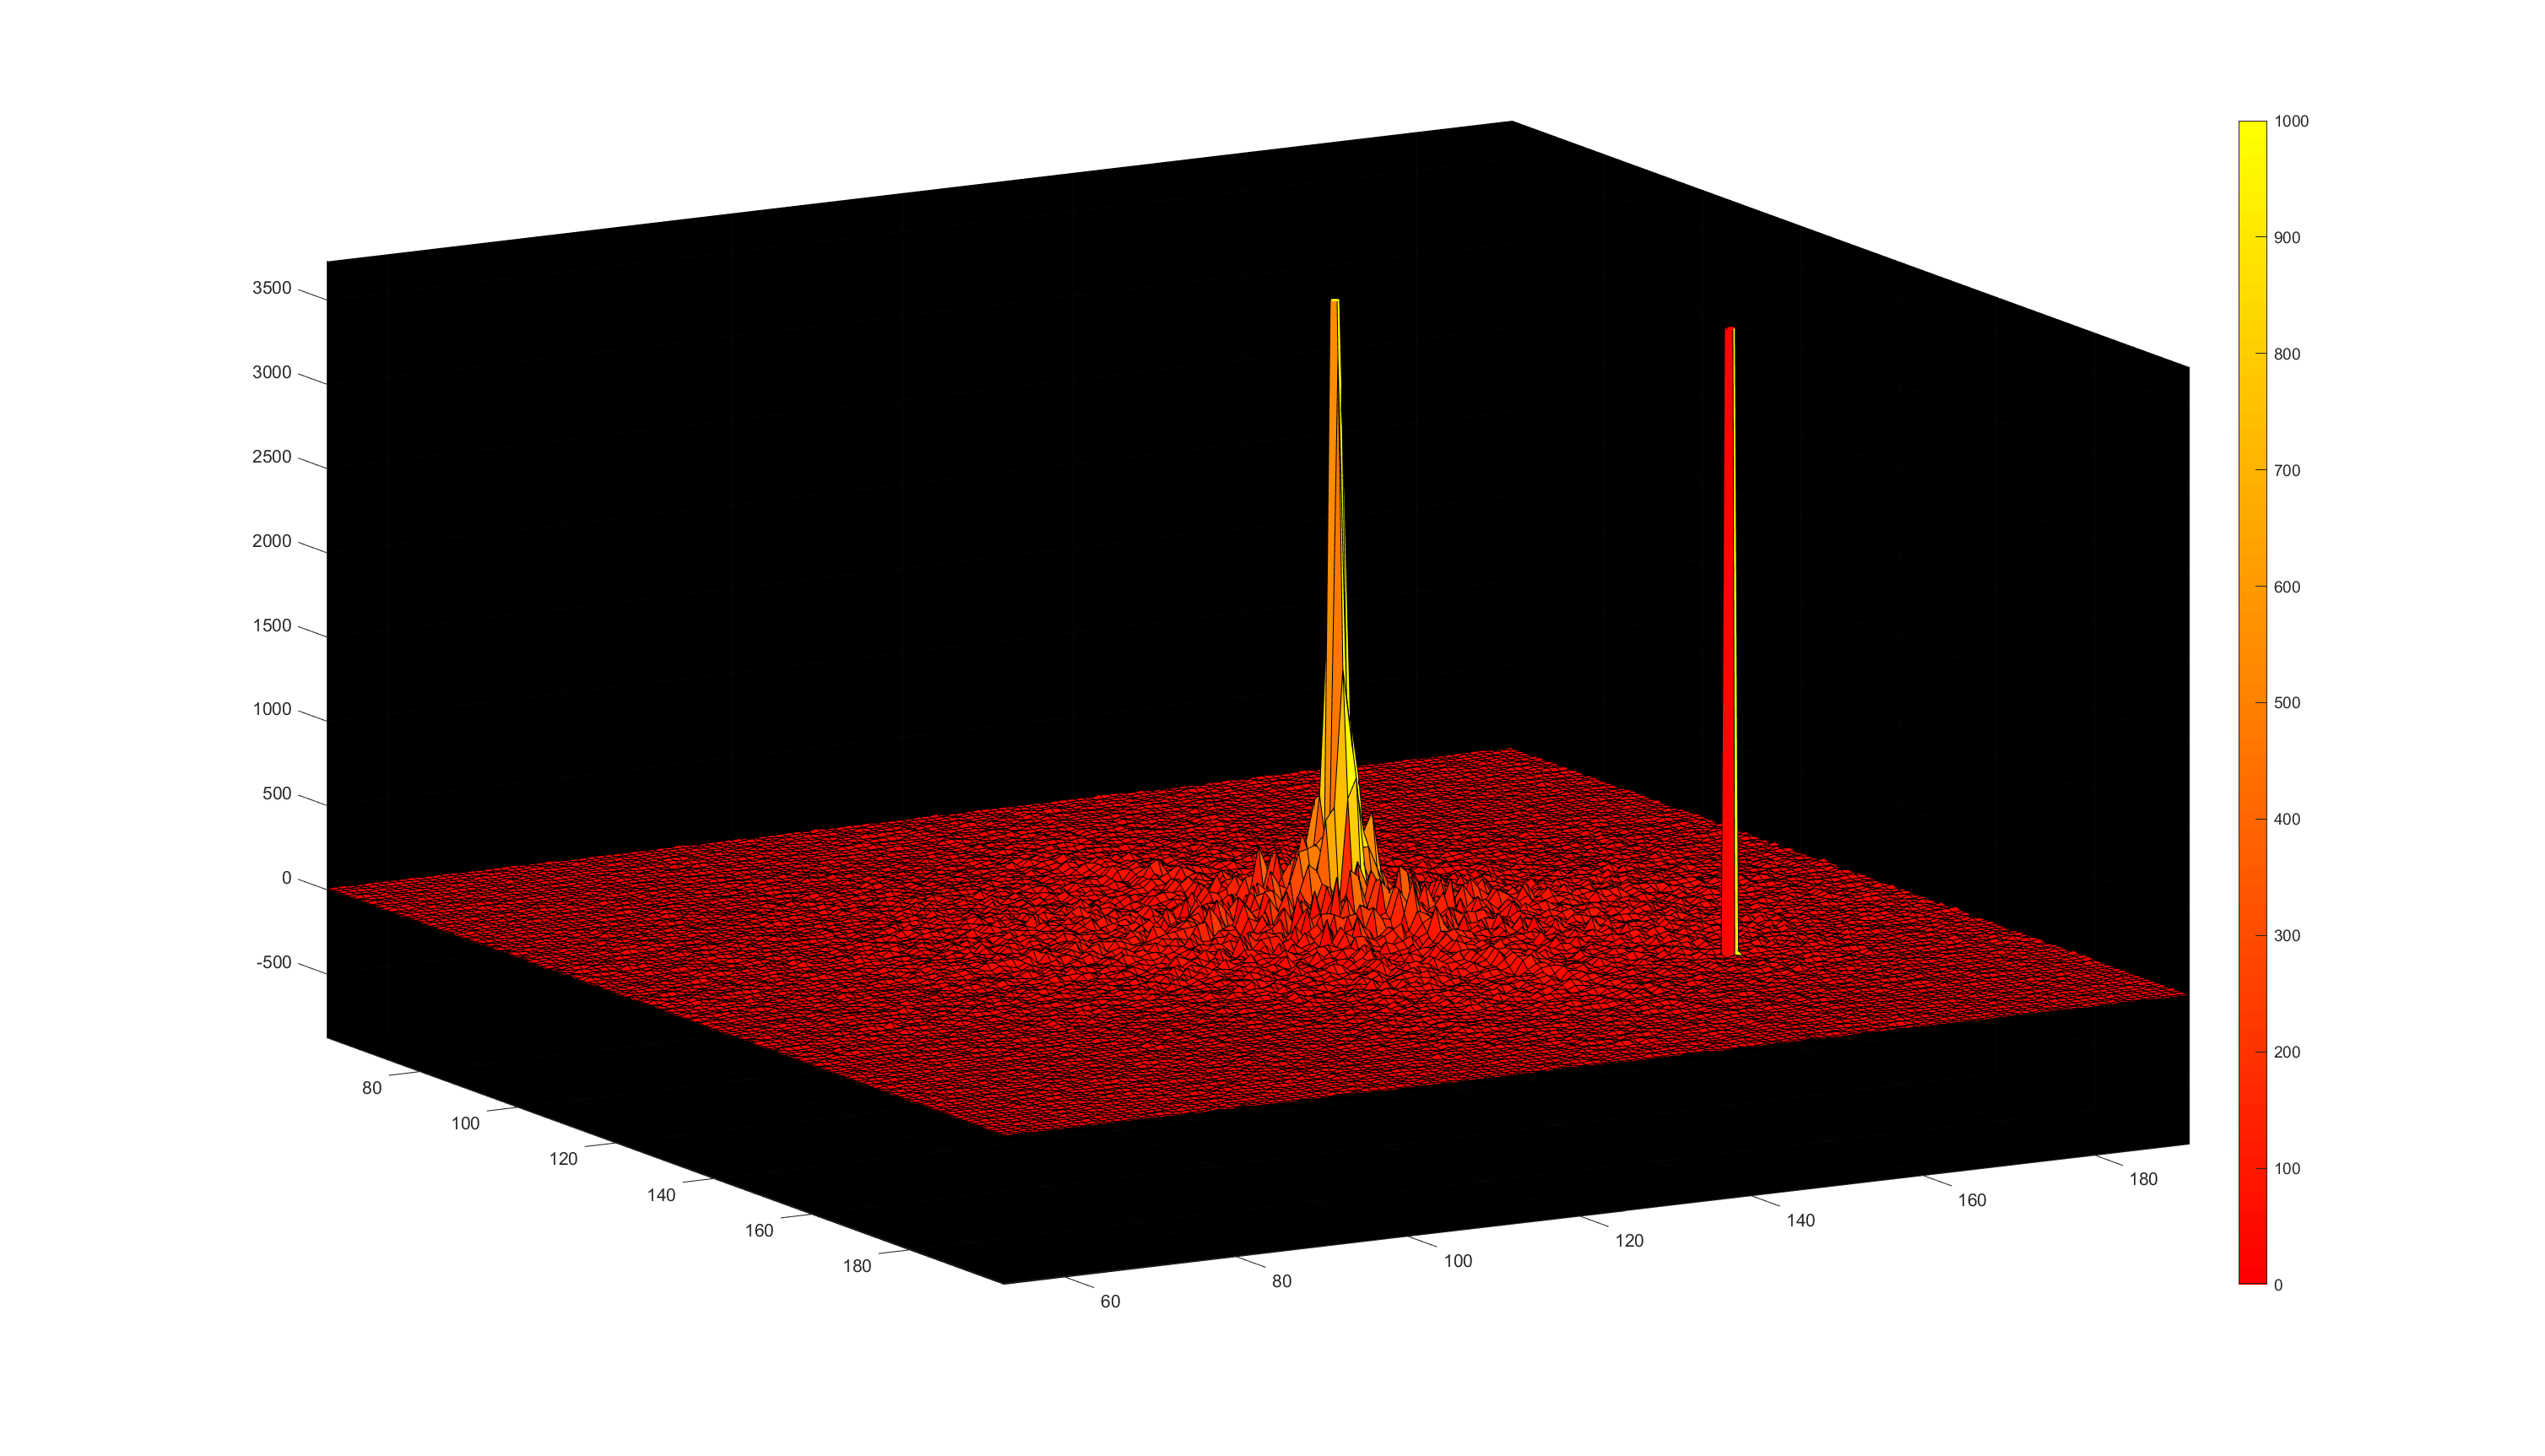
\includegraphics[width=\linewidth] {./homework4/img/Spike3d.eps}
    \caption{Magnitude plot of a changed pixel in k-space at (160,160)}
    \label{fig:recon_phase}
\end{figure}


\begin{figure}[h!]
    \centering
    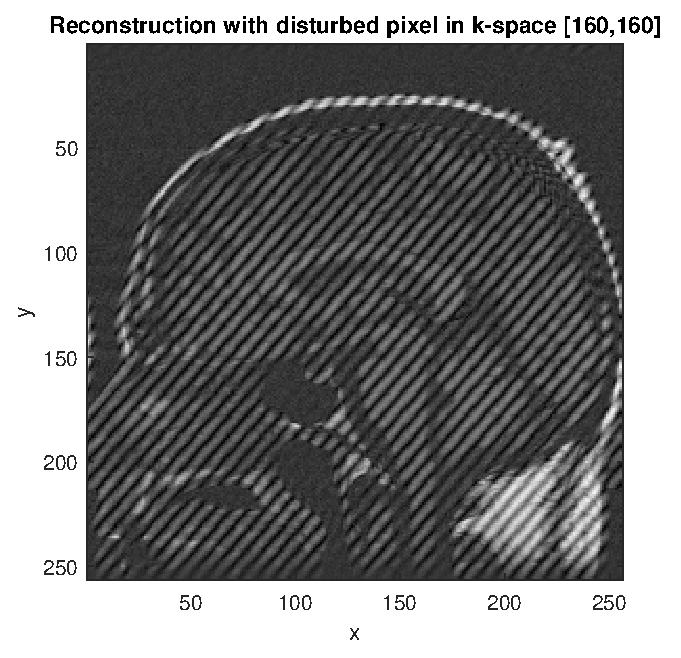
\includegraphics[width=.8\linewidth] {./homework4/img/recon_pixelanomaly.eps}
    \caption{Reconstructed image with a changed pixel in k-space at (160,160)}
    \label{fig:recon_phase}
\end{figure}



\begin{lstlisting}
%% disturb pixel (160,160)
disturbed_kspace = rawkspace;
disturbed_kspace(160,160) = 10^4;
disturbed_img = ifft2c(disturbed_kspace);
figure;
imagesc(abs(disturbed_img));
colormap(gray);
axis equal tight;
title('Reconstruction with disturbed pixel in k-space [160,160]');
xlabel('x');
ylabel('y');
print('img/recon_pixelanomaly.eps','-depsc');
\end{lstlisting}




\subsubsection{Introduce a stripe artifact in k-space, by setting the complex signal for all pixels at
column 160 equal to $\mathbf{10^2}$. Reconstruct the MR image. How do k-space stripe artifacts appear
in image space?}
Because frequency encodes for one spatial dimension, we get a line along a certain position along that spatial dimenstion. This is mostly caused by RF contamination.
A vertical stripe artifact in k-space appears as a stripe in image space:

\begin{figure}[h!]
    \centering
    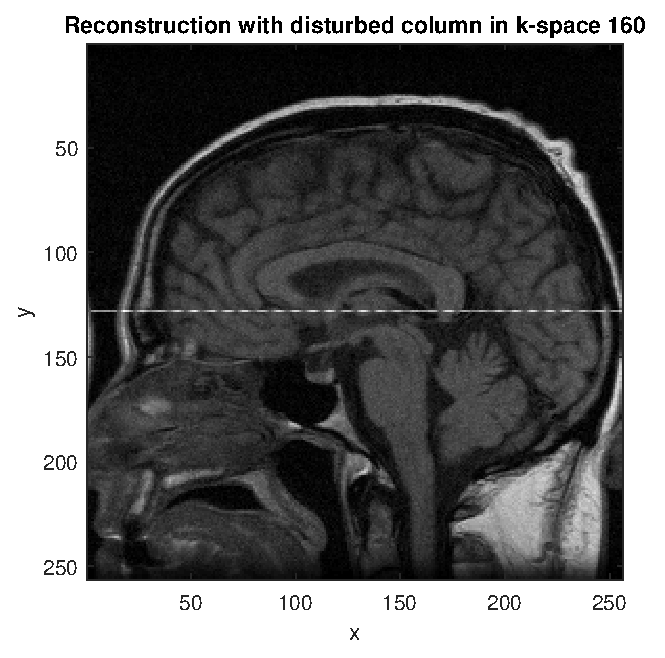
\includegraphics[width=.8\linewidth]{./homework4/img/recon_columnanomaly.eps}
    \caption{Reconstructed image with every entry in column 160 set to 100}
    \label{fig:recon_phase}
\end{figure}



\begin{lstlisting}
%% disturb column 160
disturbed_kspace2 = rawkspace;
disturbed_kspace2(:,160) = 10^2;
disturbed_img2 = ifft2c(disturbed_kspace2);

figure;
imagesc(abs(disturbed_img2));
colormap(gray);
axis equal tight;
title('Reconstruction with disturbed column in k-space 160');
xlabel('x');
ylabel('y');
print('img/recon_columnanomaly.eps','-depsc');
\end{lstlisting}




\subsubsection{Measure the noise by computing the standard deviation in a signal-less region in the
image. Display the image in SNR units, and add a colorbar to show the SNR scale.}

\begin{figure}[h!]
    \centering
    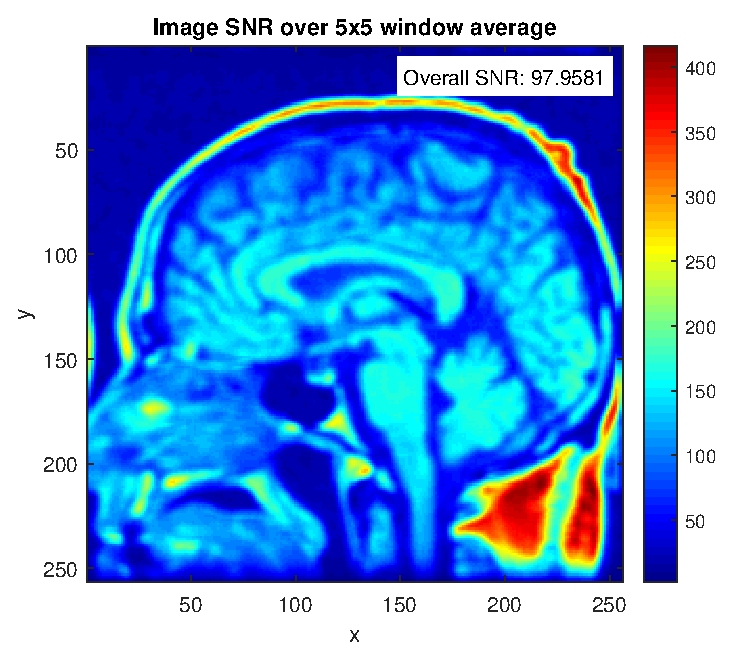
\includegraphics[width=\linewidth]{./homework4/img/recon_snr.eps}
    \caption{SNR of the reconstructed image}
    \label{fig:recon_phase}
\end{figure}




\begin{lstlisting}
%% SNR in signal
img = ifft2c(rawkspace);
% calculate SNR from small window with no signal
y_inn = 1;
y_outn = 50;
x_inn = 1;
x_outn = 50;
small_window = abs(img(y_inn:y_outn,x_inn:x_outn));
standard_deviation = std(std(small_window));
overall_SNR = mean(mean(abs(img)))/standard_deviation
% % SNR measurements
% % original data
y_ins=110;
y_outs=115;
x_ins=90;
x_outs=95;
y_inn=1;
y_outn=50;
x_inn=1;
x_outn=50;
SNRorig = mean(mean(abs(img(y_ins:y_outs,x_ins:x_outs))))/...
    std(std(abs(img(y_inn:y_outn,x_inn:x_outn))))
% SNR has been defined as the ratio of the average signal value to the
% standard deviation
% average signal over 5x5 window
average_mask = fspecial('average', 5);
averaged_image = imfilter(abs(img), average_mask);
% devide by standard_deviation
SNRorig = averaged_image/standard_deviation;
figure;
imagesc(SNRorig);
colormap(jet);
axis equal tight;
colorbar
title('Image SNR over 5x5 window average');
xlabel('x');
ylabel('y');
textColor = 'black';
textBackground = 'white';
text(200, 15, ...
['Overall SNR: ', num2str(overall_SNR) ], ...
'Color', textColor, ...
'BackgroundColor', textBackground, ...
'HorizontalAlignment', 'Center');
print('img/recon_snr.eps','-depsc');
\end{lstlisting}





\subsubsection{Zero-fill the k-space data to a 512x512 matrix by symmetrically adding zeros around
the data. This will interpolate the image to a larger matrix size. Reconstruct the image,
compute the SNR, and display in SNR units.}
Adding zeros around the image increases the field of view

\begin{figure}[h]
    \centering
    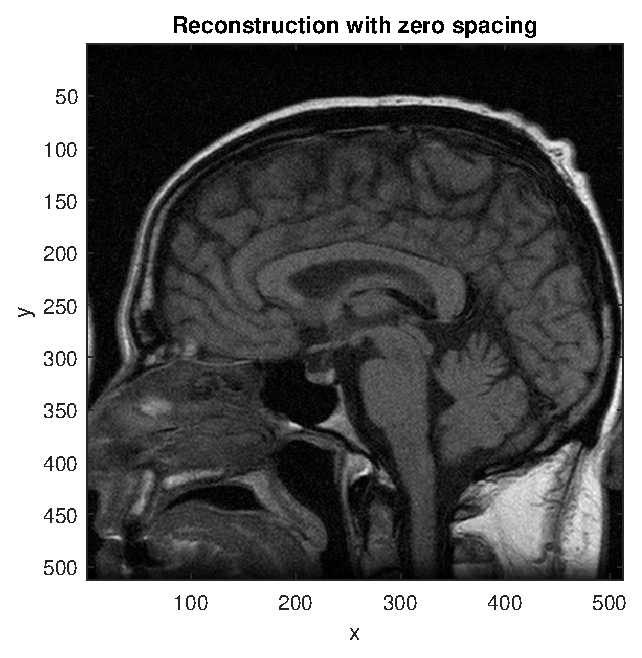
\includegraphics[width=.85\linewidth] {./homework4/img/recon_zerofilled.eps}
    \caption{Reconstructed image from an enlarged, zero-filled k-space}
    \label{fig:recon_zero}
    \end{figure} 
    
    \begin{figure}[h]
    \centering
    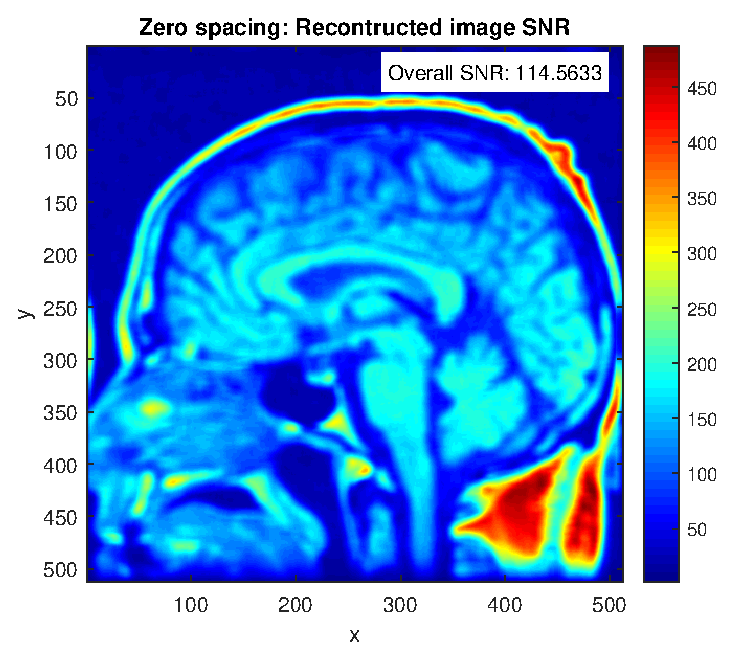
\includegraphics[width=\linewidth] {./homework4/img/recon_zerofilledSNR.eps}
    \caption{SNR from figure \ref{fig:recon_zero}}
    \label{fig:recon_zeroSNR}
    \end{figure}
\clearpage



\begin{lstlisting}
%% zero-filling to 512x512
% image 512
rawkspacefill = zeros(512,512);
rawkspacefill((1:256) + 128,(1:256) + 128) = rawkspace;
imfill = ifft2c(rawkspacefill);
% reconstruct the imagefigure;
imagesc(abs(imfill));
colormap(gray);axis equal tight;
title('Reconstruction with zero spacing');
xlabel('x');
ylabel('y');
print('img/recon_zerofilled.eps','-depsc');
% now SNR of image --> double size of window and filter
y_inn = 1;
y_outn = 100;
x_inn = 1;
x_outn = 100;
small_window = abs(imfill(y_inn:y_outn,x_inn:x_outn));
standard_deviation_2 = std(std(small_window));
%overall SNR
overall_SNR_imfill = mean(mean(abs(imfill)))/standard_deviation_2;
average_mask = fspecial('average', 10);
averaged_imfill = imfilter(abs(imfill), average_mask);
% devide by standard_deviation
SNRimfill = averaged_imfill/standard_deviation_2;
figure;
imagesc(SNRimfill);
colormap(jet);
axis equal tight;
colorbar
title('Zero spacing: Recontructed image SNR');
xlabel('x');
ylabel('y');
textColor = 'black';
textBackground = 'white';
text(390, 25, ...
['Overall SNR: ', num2str(overall_SNR_imfill) ], ...
'Color', textColor, ...
'BackgroundColor', textBackground, ...
'HorizontalAlignment', 'Center');
print('img/recon_zerofilledSNR.eps','-depsc');
\end{lstlisting}





\subsubsection{Windowing: Multiply the data by a 2D Hanning window. Reconstruct the image,
compute the SNR, and display in SNR units. How has the SNR changed? How has the
image changed? How are these changes related?}
The resolution becomes worse, the image is more blurry.
By Hanning-filtering, we amplify low frequencies in k-space and squeeze the high frequencies together. Hence, we are removing fine
details, but also the noise. It improves the SNR and makes medium-sized features better visible, but lowers the resolution.


\begin{figure}[h]
    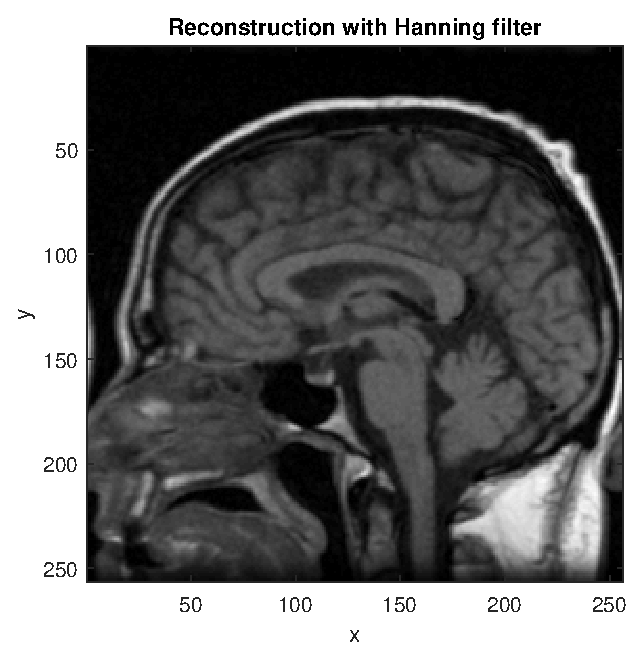
\includegraphics[width=.85\linewidth] {./homework4/img/recon_hanning.eps}
    \caption{Reconstructed image with a 2D hanning filtering.}
    \label{fig:recon_hanning}
    \end{figure} 
    
    \begin{figure}[h]
    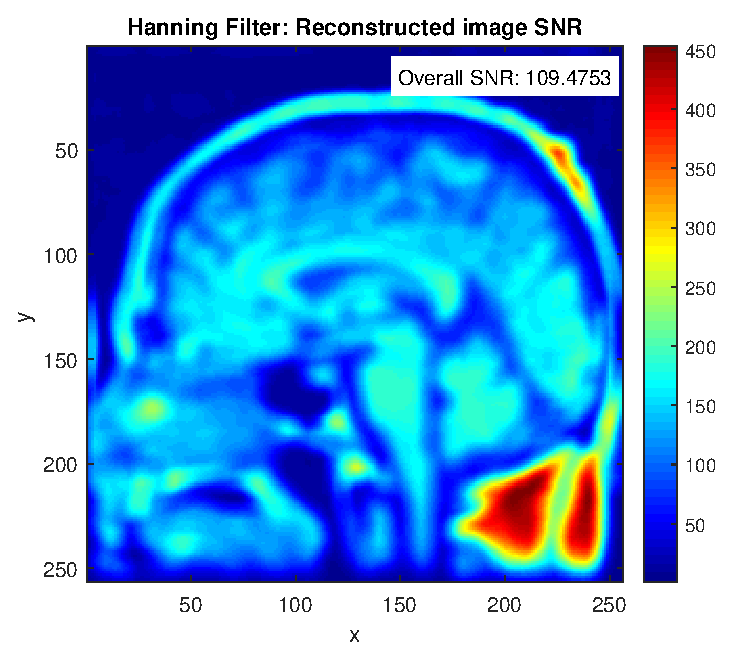
\includegraphics[width=\linewidth] {./homework4/img/recon_hanningSNR.eps}
    \caption{SNR of figure \ref{fig:recon_hanning}}
    \label{fig:recon_hanningSNR}
    \end{figure}

\clearpage

\begin{lstlisting}
%% Hanning window
% hanning window in k-space
rawkspace_hann = rawkspace.* (hann(256)* hann(256)');
ima_hann = ifft2c(rawkspace_hann);
%reconstruct image
figure;
imagesc(abs(ima_hann));
colormap(gray);axis equal tight;
title('Reconstruction with Hanning filter');
xlabel('x');
ylabel('y');
print('img/recon_hanning.eps','-depsc');
% calculate SNR from small window with no signal
y_inn=1; y_outn=50;
x_inn=1; x_outn=50;
small_window_hann = abs(ima_hann(y_inn:y_outn,x_inn:x_outn));
standard_deviation_hanning = std(std(small_window_hann));
overall_SNR_hanning = mean(mean(abs(ima_hann)))/standard_deviation_hanning;
% SNR has been defined as the ratio of the average signal value to the
% standard deviation
% average signal over 5x5 window
average_mask_hann = fspecial('average', 5);
averaged_image = imfilter(abs(ima_hann), average_mask);
% devide by standard_deviation
SNRhann = averaged_image/standard_deviation_hanning;
figure;
imagesc(SNRhann);
colormap(jet);
axis equal tight;
colorbar
title('Hanning Filter: Reconstructed image SNR');
xlabel('x');
ylabel('y ');
textColor = 'black';
textBackground = 'white';
text(200, 15, ...
['Overall SNR: ', num2str(overall_SNR_hanning) ], ...
'Color', textColor, ...
'BackgroundColor', textBackground, ...
'HorizontalAlignment', 'Center');
print('img/recon_hanningSNR.eps','-depsc');
\end{lstlisting}




    % \subsection{Task}
    % \begin{figure}
    % \begin{minipage}{\textwidth}
    % 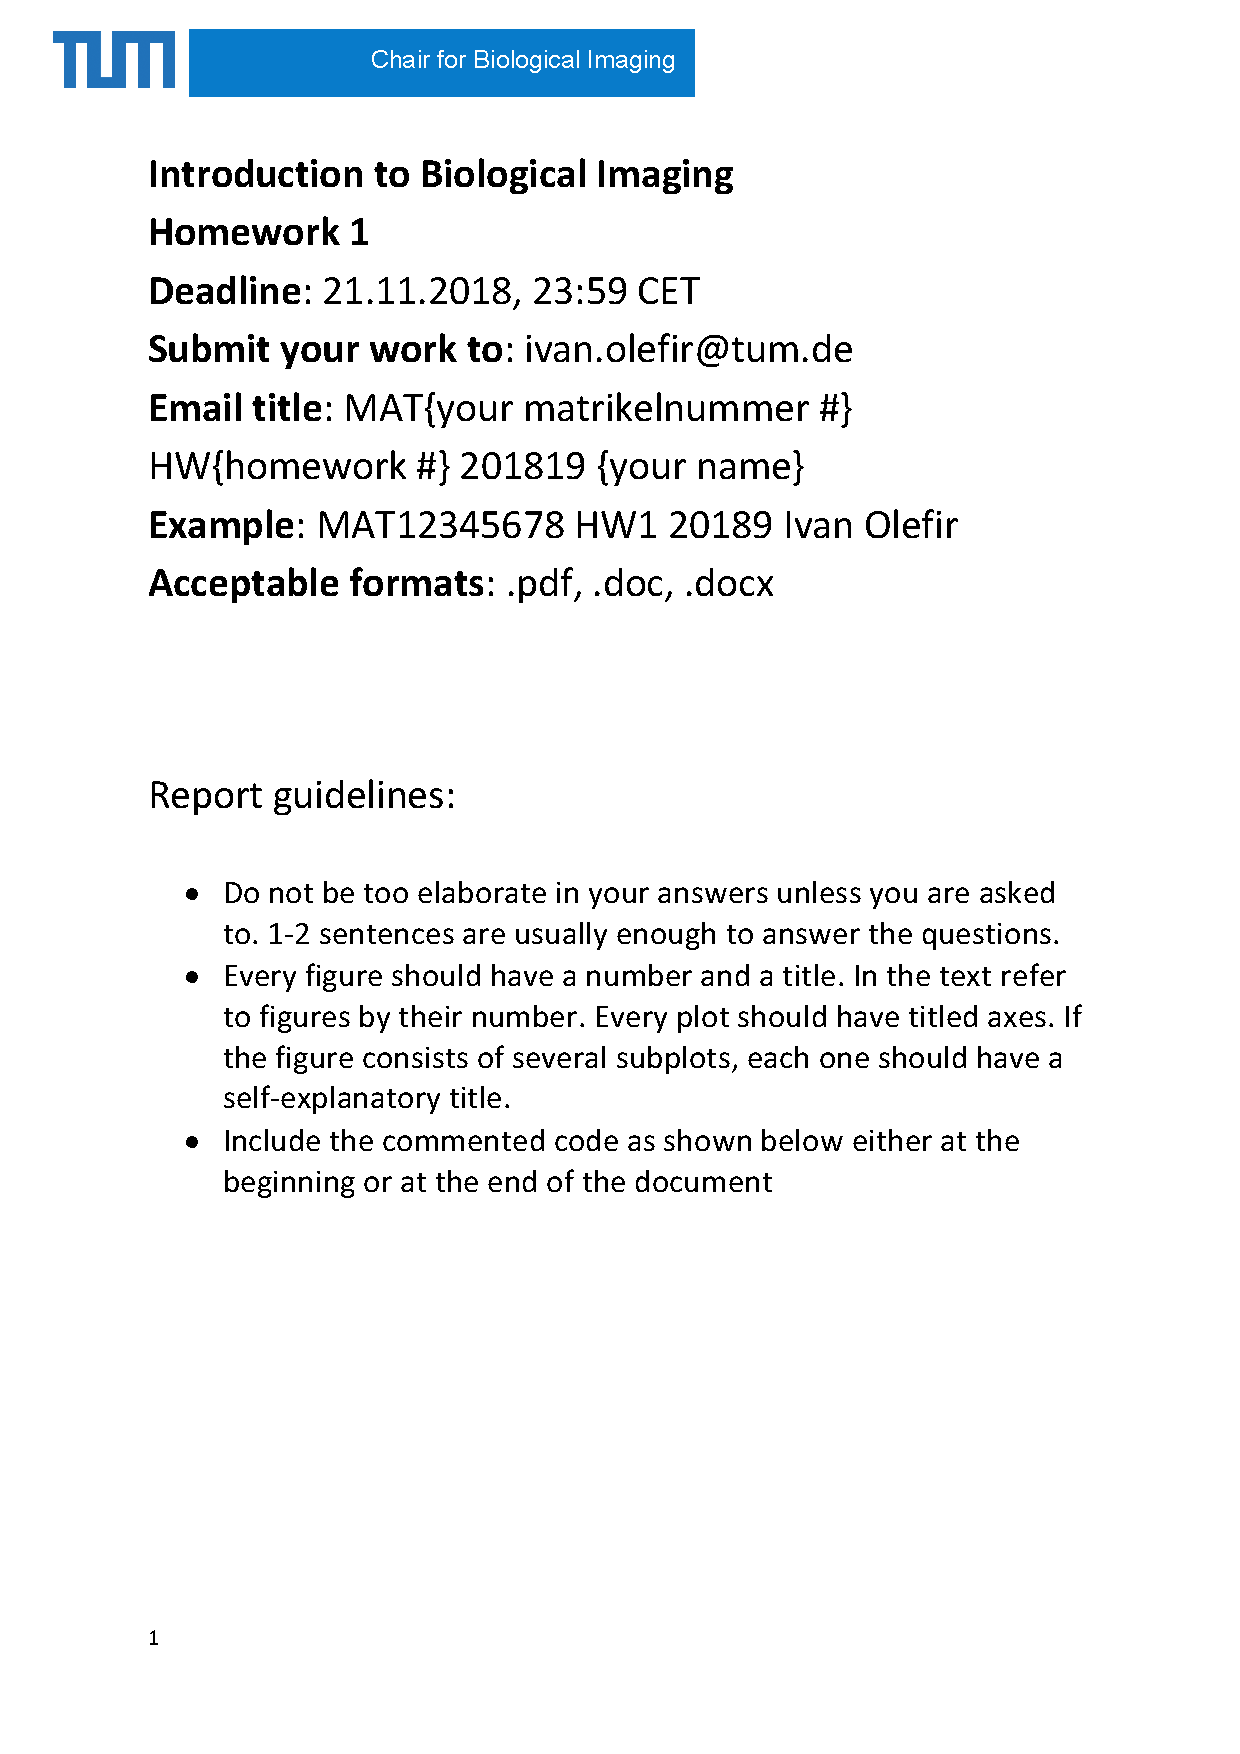
\includepdf[
    %     trim=2.2cm 8cm 2.2cm 2.2cm,
    %     clip,
    %     pages=-2,
    %     nup=2x1,
    %     frame,
    %     scale=0.7,
    %     pagecommand={}
    %  ]{Homework1_2018.pdf} 
    %  \end{minipage}
    %  \end{figure}
    % \includepdf[
    %     trim=2.2cm 2.2cm 2.2cm 2cm,
    %     clip,
    %     pages=3-,
    %     nup=2x1,
    %     frame,
    %     scale=0.8,
    %     pagecommand={}
    %  ]{Homework1_2018.pdf}
    
    


\end{document}
